\chapter{Entropia}

\section{Definizione di entropia}

\begin{definizione}[entropia]
Si dice \textit{entropia} il contenuto informativo medio di una sorgente S.
\end{definizione}

Dato un generico evento E come possiamo materialmente definire il contenuto informativo I(E) di questo evento? Shannon parte dalla considerazione che l'osservatore ha un patrimonio di conoscenze acquisite e di conseguenza ha una certa idea della probabilità che tale evento si verifichi. L'idea di base è che il contenuto informativo ha a che fare con l'incertezza: più l'osservatore è sorpreso nel 
vedere un simbolo, più il livello di contenuto informativo sarà alto (e viceversa).
Quindi più la probabilità di un evento è bassa, più sarà alto il suo I(E) se tale evento si verifica, fino ad arrivare all'estremo di un evento con probabilità prossima a 0, che avrà un contenuto informativo tendente a infinito.

Possiamo quindi dire che il contenuto informativo di un evento sarà funzione della sua probabilità:
\[I(E) = f(P(E))\]
Proviamo ora a enumerare quali proprietà debba avere la funzione f affinchè il ragionamento fatto finora abbia senso:
\begin{enumerate}
\item f dovrebbe essere definita nell'intervallo \((0,1]\) (aperto a sinistra). Infatti l'argomento di f è una probabilità (che per 
definizione è compresa tra 0 e 1). Inoltre escludiamo lo 0, in quanto in tal caso l'evento non si verifica mai e non è quindi di interesse. Si deve quindi avere:
\[f: (0,1] \longrightarrow \R^+\]
\item f(1) = 0, in quanto l'evento certo non porta nessuna informazione
\item $\lim_{P(E) \rightarrow 0} f(P(E)) = + \infty$
      In quanto quando la probabilità tende a 0, abbiamo il massimo contenuto informativo (c'è la massima ``sorpresa'').
\item f sarà una funzione continua, in quanto non ci aspettiamo che ci siano dei ``salti'' di probabilità
\item f sarà una funzione monotona decrescente (strettamente)
\item consideriamo 2 eventi indipendenti \(E_1\) ed \(E_2\) (esempio: ``oggi c'è il sole'' ed ``è uscita testa dal lancio di una moneta'') , il contenuto informativo dell'intersezione dei due eventi \(I(E_1 \cap E_2)\) (l'evento congiunto) è dato dalla somma dei rispettivi contenuti informativi:
\[I(E_1 \cap E_2) = I(E_1) + I(E_2)\]
Esprimendo il contenuto informativo utilizzando la funzione f, e tenendo conto che la probabilità dell'evento congiunto è pari al prodotto della probabilità dei singoli eventi otteniamo:
\[
\begin{split}
I(E_1 \cap E_2) &= f(P(E_1 \cap E_2)) \\
&= f(P(E_1) \cdot P(E_2)) 
\end{split}
\]
quindi dovrà essere:
\[I(E_1) + I(E_2) = f(P(E_1) \cdot P(E_2))  \]
ossia (sintesi finale della proprietà):
\[ f(P(E_1) \cdot P(E_2)) = f(P(E_1)) + f(P(E_2)) \]
\end{enumerate}

Una funzione che permette di rispettare la proprietà 6 è il logaritmo (\ref{fig:0010}), in quanto il logaritmo del prodotto di due termini è pari alla somma dei logaritmi dei singoli termini, ma tale funzione non rispetta la proprietà 3. Possiamo però prendere la funzione \(- \log x\) (figura \ref{fig:0011}): questa rispetta tutte le proprietà, per cui Shannon ha definito il \textbf{contenuto informativo di un evento} come \(- \log P(E)\), oppure come \(\log \frac{1}{P(E)}\) (semplice proprietà dei logaritmi).
Shannon dimostra anche che questa funzione è l'unica in grado di rispettare tutte le proprietà.

\begin{figure}[htbp]
\begin{center}
	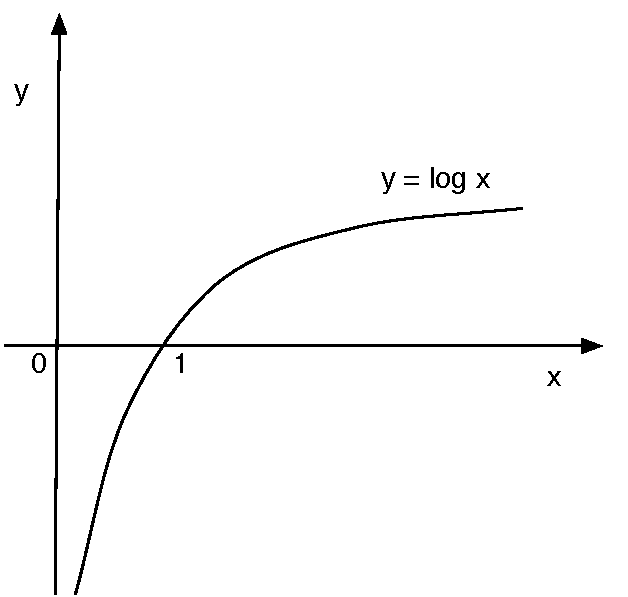
\includegraphics[width=0.6\textwidth]{img/logx.pdf}
\caption{funzione logaritmo}
\label{fig:0010}
\end{center}
\end{figure}

\begin{figure}[htbp]
\begin{center}
	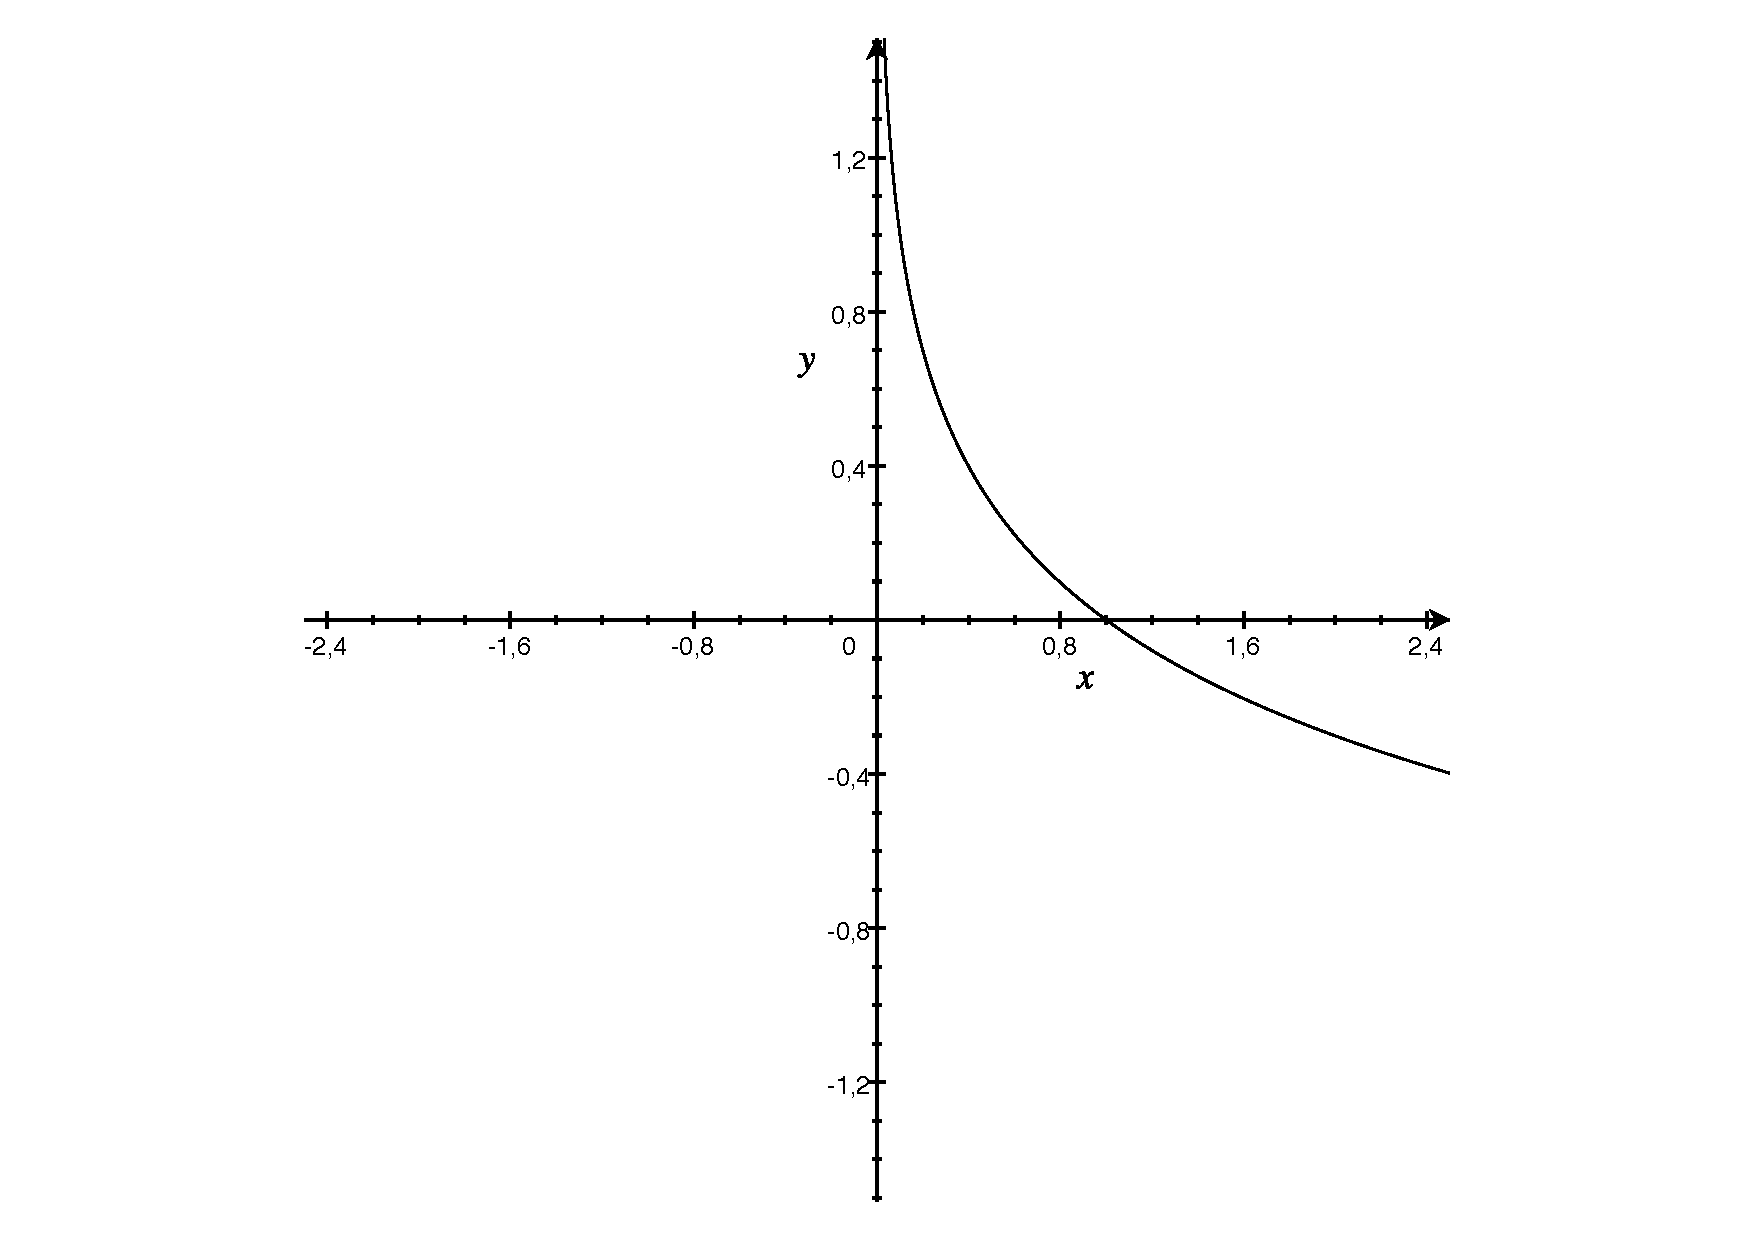
\includegraphics[width=0.6\textwidth]{img/logx2.pdf}
\caption{funzione \(- \log(x)\)}
\label{fig:0011}
\end{center}
\end{figure}

Abbiamo così definito il contenuto informativo di un singolo evento, dobbiamo invece cercare di esprimere il \textbf{contenuto informativo medio} della sorgente. Supponiamo quindi di avere una sorgente che genera una sequenza di simboli \(s_1, s_2, s_3 ... s_n\). Ciascun evento (ovvero simbolo generato) ha contenuto informativo pari a \(I(s_1), I(s_2) ... I(s_n) = -\log p(s_1), -\log p(s_2) ... -\log p(s_n)\). Il contenuto informativo medio della sorgente sarà quindi la media dei contenuti informativi dei singoli eventi:
\[
\begin{split}
H(S) &= \sum_{s \in S} p(s) I(s)\\
&= - \sum_{s \in S} p(s) \log p(s)\\
&= \sum_{s \in S} p(s) \log \frac{1}{p(s)}
\end{split}
\]

In maniera del tutto equivalente, possiamo descrivere la sorgente con una variabile aleatoria (v.a.).
In particolare possiamo considerare la v.a. X, tale che \(\X = \{x_1, x_2 ... x_n\}\).
La probabilità che si verifichi l'evento x è:
\[P\{X = x\} = p(x) \ x \in \X\]
allora il contenuto informativo per tale evento è:
\[I\{X = x\} = - \log p(x)\]
In maniera analoga a prima, il contenuto informativo medio sarà dato dal valore atteso della variabile X.
Questa quantità è proprio l'entropia H(X) (si noti che questo concetto non ha nulla a che fare con quello di entropia della fisica).

\noindent
Formalmente:
\begin{definizione}
\[H(X) \triangleq - \sum_{x \in \X} p(x) \log p(x) = \sum_{x \in \X} p(x) \log \frac{1}{p(x)}\]
\end{definizione}

A questo punto dobbiamo definire l'unità di misura che utilizzeremo. Infatti, al variare della base del logaritmo, cambia 
il valore numerico dell'entropia. In tabella \ref{tab:0001} sono riportate le principali basi utilizzate, con la relativa unità di misura.

\begin{table}[htbp]
	\begin{center}
	\begin{tabular}{ccc}
		\toprule
		Base & Unità di misura \\ 
		\midrule 
		2    & bit             \\ 
		e    & nat             \\ 
		10   & Hartley         \\ 
		\bottomrule               
	\end{tabular}
	\caption{unità di misura utilizzate e basi corrispondenti}
	\label{tab:0001}
	\end{center}
\end{table}

\noindent
Possiamo convertire da una misura all'altra utilizzando la formule dei logaritmi per il cambio di base:
\[\log_b x = \frac{\log_a x}{\log_a b}\]

\noindent
Se si vuole indicare una entropia in una specifica base, si può utilizzare la seguente definizione:
\begin{definizione}[entropia con base a]
Definiamo l' \textit{entropia con base a} come:
\[H_a(X) = - \sum_{x \in \X} p(x) \log_a p(x)\]
\end{definizione}

E' a questo punto necessaria una precisazione riguardante la definizione di entropia che è stata data.
Se supponiamo infatti di avere uno o più simboli dell'alfabeto che non verranno mai generati, si 
hanno degli x per i quali \(p(x) = 0\).
Succede dunque che nel calcolo dell'entropia ci si trova di fronte al calcolo di \(\log 0\), che non è definito.

\noindent
Possiamo però calcolare il limite della quantità in questione:
\[\lim_{p(x) \rightarrow 0} p(x) \log(p(x))\]
\[=\lim_{x \rightarrow 0} \frac{\log p(x)}{\frac{1}{p(x)}}\]
applicando la regola di de l'Hôpital:
\[\lim_{p(x) \rightarrow 0} \frac{\frac{1}{p(x)}}{-\frac{1}{p(x)^2}} = \lim_{p(x) \rightarrow 0} p(x) = 0\]

Per ovviare quindi al precedente problema poniamo \(0 \log 0 = 0\).
Questo ci consente di non considerare le probabilità nulle, in quanto non hanno alcuna influenza sul valore 
dell'entropia.







\section{Studio della funzione entropia}
Risulta utile studiare la funzione entropia (lo faremo in un caso particolare), in maniera tale da avere una idea precisa del suo comportamento.
Innanzitutto però facciamo due osservazioni:
\begin{enumerate}
\item l'entropia è sempre maggiore o uguale a 0:
\[H(x) \geq 0\]
questo perché:
\[H(x) = - \sum_{x \in \X} p(x) \log p(x)\]
ma sappiamo che \(p(x) \geq 0\) e che \(\log p(x) \leq 0\), quindi nel complesso \(p(x) \log p(x)\) sarà sempre negativo, essendoci il segno meno all'esterno della sommatoria, risulta che l'entropia è sempre maggiore o uguale a 0.

\item possiamo cambiare la base dell'entropia (dalla base a alla base b) tramite la seguente formula:
\[H_b(X) = \log_b a \cdot H_a(X) = \frac{H_a(X)}{\log_a b}\]
La dimostrazione è banale, utilizzando la proprietà del cambio di base dei logaritmi.
\end{enumerate}

Prendiamo ora l'esempio di una variabile aleatoria X associata al lancio di una moneta bilanciata, che assume quindi solo i valori 0 (testa) e 1(croce):
\[\X = \{0,1\}\]
\[P\{X = 0\} = 1/2\]
\[P\{X = 1\} = 1/2\]
Si tratta del caso peggiore in quanto non possiamo fare previsioni sul prossimo simbolo emesso, poiché entrambi hanno la stessa probabilità. Vediamo quanto vale l'entropia in questo caso:
\[
\begin{split} 
H(X) &= - P(X = 0) \cdot \log P(X = 0) - P(X = 1) \cdot \log P(X = 1)\\ 
&= -\frac{1}{2} \log{\frac{1}{2}} -\frac{1}{2} \log{\frac{1}{2}}\\ 
&= - \frac{1}{2} \log{2^{-1}} - \frac{1}{2} \log{2^{-1}}\\
&= - \frac{1}{2} (-1) \log{2} - \frac{1}{2} (-1) \log{2}\\
&= \frac{1}{2} \log{2} + \frac{1}{2} \log{2} = 1 bit
\end{split} 
\]
Abbiamo quindi anallizzato solo il caso particolare in cui la moneta è bilanciata, ovvero il caso in cui le probabilità di generazione dei vari simboli siano tutte uguali. Proviamo ora a generalizzare la nostra analisi prendendo in esame la famiglia di sorgenti binarie, introducento un parametro p. Tale parametro esprimere la probabilità di generazione dei 2 simboli (al variare di p ottengo sorgenti diverse):
\[X \ v.a. \qquad \X = \{0,1\}\]
\begin{align*}
p(0) &= P(X = 0) = p \quad 0 \leq p \leq 1 \\
p(1) &= P(X = 1) = 1-p
\end{align*}
Calcolando l'entropia generalizzata:
\[H(p) = - p \log{p} -(1-p) \log (1-p) \mbox{ con } p \in [0,1]\]

\noindent
Studiamo ora il comportamento di questa funzione (figura \ref{fig:entropia}).

\noindent
Osserviamo che:
\begin{enumerate}
\item qualsiasi entropia è sempre maggiore o uguale a 0
\item negli estremi dell'intervallo la funzione assume valori (ricordando che abbiamo posto \(0 \log 0 = 0\)):
\[H(0) = - 0 \log{0} -(1-0) \log (1-0) = 0\] 
\[H(1) = - 1 \log{1} -(1-1) \log (1-1) = 0\]
dall'esempio precedente sappiamo inoltre che \(H(1/2) = 1\);
\item si può notare una certa simmetria, tale che \(H(p) = H(1-p)\) infatti:
\[
\begin{split}
H(1-p) &= - (1- p) \log{(1-p)} -(1- 1 + p) \log (1- 1 + p) \\
&= - (1- p) \log{(1-p)} - p \log p = H(p)
\end{split}
\]
\item studiando la derivata possiamo capire quali siano i punti di minimo e massimo:
\[
\begin{split} 
D \ H(p) &= \frac{d H(p)}{d p} \\ 
&= - \frac{d [p \log p + (1-p) \log (1-p)]}{d p} \\ 
&= - [\log p + \cancel{p} \frac{1}{\cancel{p}} \log e - \log{(1-p)} - \cancel{(1-p)} \frac{1}{\cancel{(1-p)}}\log e] \\ 
&= - [\log p +  \cancel{\log e} - \log{(1-p)} - \cancel{\log e}] \\ 
&= \log (1-p) - \log p \\ 
\end{split} 
\]
per trovare i punti di massimo è sufficiente controllare quando si annulla la derivata:
\[\frac{d H(p)}{d p} = 0 \Longrightarrow \log (1-p) \cdot \log p = 0 \iff 1-p = p \iff p = 1/2\]
Quindi c'è un unico punto in cui si annulla, ossia il massimo valore assunto dall'entropia è:
\[H(1/2) = 1\]
\item H(p) è concava\footnote{
\begin{definizione}[funzione convessa]
Data la funzione:
\[f: [a,b] \longrightarrow \R \]
f si dice \textit{funzione convessa} se
\[\forall x_1, x_2 \in [a,b], \lambda \in [0,1] \quad f(\lambda x_1 + (1-\lambda)x_2) \leq \lambda f(x_1) + (1-\lambda) f(x_2)\]
\end{definizione}

\begin{definizione}[funzione concava]
Data la funzione:
\[f: [a,b] \longrightarrow \R \]f si dice \textit{funzione concava} se -f è convessa.
\end{definizione}
} per il teorema descritto nella nota a piè di pagina\footnote{
\begin{teorema}
se \(f \in \E^1\) (ossia se f è derivabile almeno 1 volta) allora:
\[\mbox{f convessa} \iff \forall x, x_0 \in [a,b] : f(x) \geq f(x_0) + f'(x_0) (x-x_0)\]
\label{concava1}
\end{teorema}

\begin{teorema}
se \(f \in \E^2\) (ossia se f è derivabile almeno 2 volte) allora:
\[\mbox{f convessa} \iff \forall x \in [a,b]: f''(x) \geq 0\]
\label{concava}
\end{teorema}
}, infatti:
\[
\begin{split} 
H''(p) &= \frac{d^2 H(p)}{dp^2} = \\ 
&= \frac{d [\log(1-p) - \log p]}{dp} \\ 
&= - \frac{1}{1-p}\log e - \frac{1}{p} \log e < 0 \ \forall \ p \in [0,1]
\end{split} 
\]
in quanto per \(p \in [0,1]\) sia \(- \frac{1}{1-p}\) sia \(- \frac{1}{p}\) sono negativi;
\item la funzione è simmetrica rispetto all'asse verticale \(p = \frac{1}{2}\); per dimostrarlo deve essere che \(\forall \ q \leq 1/2\):
\[H(1/2 - q) = H(1/2 + q)\]
ma sappiamo che:
\[H(p) = H(1-p)\]
quindi:
\[H(1/2 + q) = H(1-(1/2 - q)) = H(1/2 - q)\]
pertanto la funzione entropia ha una forma a campana simmetrica (figura \ref{fig:entropia}).
\end{enumerate}
Si ricordi che questo studio è stato effettuato nel caso di 2 variabili (i grafici sono infatti bidimensionali). E' possibile (sebbene 
sia abbastanza complicato), estendere quanto visto al caso generale con n variabili.

\begin{figure}[htbp]
\begin{center}
	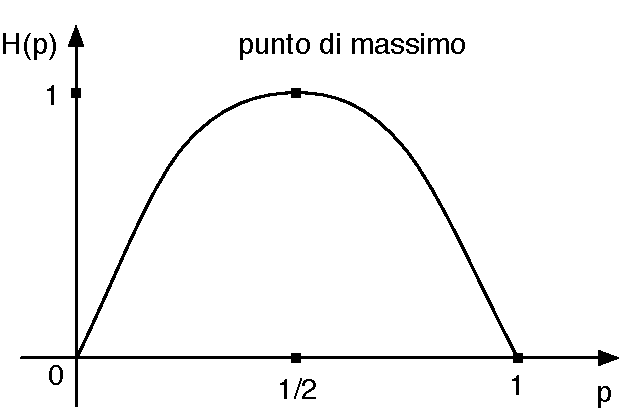
\includegraphics[width=0.6\textwidth]{img/entropia.pdf}
\caption{studio della funzione H(p)}
\label{fig:entropia}
\end{center}
\end{figure}










\section{Proposizioni sull'entropia}
Vengono ora presentate alcune proposizioni che hanno come oggetto l'entropia.
Tuttavia, per dimostrare formalmente la loro validità, sarà necessario introdurre prima 
alcuni concetti e risultati.
\subsection{Simplesso standard}

\begin{figure}[htbp]
  \centering
  \subfloat[n=2]{\label{fig:simpl2}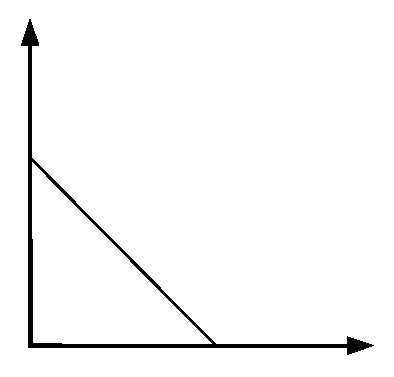
\includegraphics[width=0.4\textwidth]{img/simplex2.pdf}}                
  \subfloat[n=3]{\label{fig:simpl3}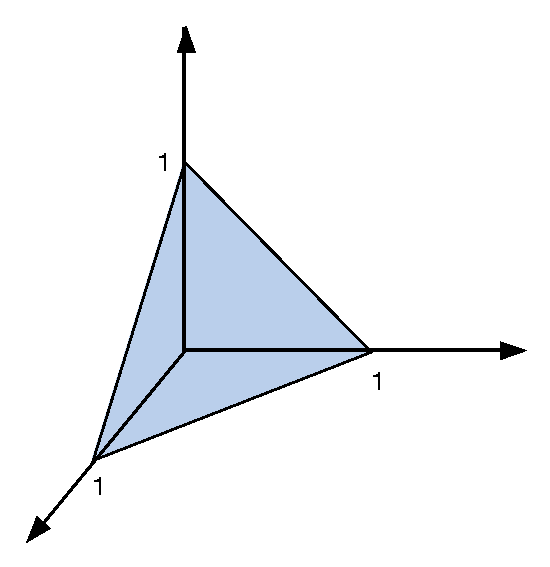
\includegraphics[width=0.4\textwidth]{img/simplex3.pdf}}
  \caption{Rappresentazione del simplesso standard}
  \label{fig:animals}
\end{figure}

Il simplesso standard di $R^n$ o spazio delle probabilità n-dimensionale, è definito come segue:
\begin{definizione}[Simplesso standard]

 \[ \triangle_n = \{ \bar{x} \in R^n \mid \sum_{i=1}^{n} x_i=1 \ ; \ \forall i=1..n: x_i \ge 0 \} \]
\end{definizione}

Per chiarire meglio il concetto, facciamo due esempi:
\begin{itemize}
 \item Nel caso in cui n=2, abbiamo il simplesso standard unidimensionale (figura \ref{fig:simpl2}).
       Deve essere che $x_1 \ge 0, x_2 \ge 0$ e che $x_1+x_2=1$. Nella figura $x_1$ è rappresentato 
       sull'asse x, mentre $x_2$ sull'asse y (l'inverso è equivalente).
       Si ottiene dunque un segmento.
 \item Nel caso in cui n=3, abbiamo il simplesso standard bidimensionale (figura \ref{fig:simpl3}).
       In questo caso si ottiene un triangolo.
\end{itemize}





\subsection{Disuguaglianza di Gibbs}
Prima di introdurre la disuguaglianza di Gibbs, presentiamo un lemma che sarà utile 
per dimostrare la validità della disuguaglianza.

\begin{lemma}

 \[ln(x) \le x-1 \] 
 \begin{proof}
  Sia $y=ln(x)$, allora $y'=\frac{1}{x}$ e $y''=-\frac{1}{x^2}$.

  Poiché $y''$ è sempre negativa, la funzione y è strettamente concava (Teorema \ref{concava}).
  Ma se una funzione è concava, per il teorema \ref{concava1} deve essere:
  \[ f(x) \le f(x_0) + f'(x_0)(x-x_0) \]
  
  Quindi per la funzione y:
  \[ ln(x) \le ln(x_0) + \frac{1}{x_0}(x-x_0) \]

  Ponendo $x_0=1$ risulta:
  \[ ln(x) \le x-1 \]
 \end{proof}
  \label{lemma_entr}
\end{lemma}

\begin{osservazione}
 Il lemma precedente può essere esteso anche al caso di un logaritmo con base qualunque.
 In particolare risulta:
 \[log(x) \le log(e)(x-1) \]
 La dimostrazione è banale e si basa sulla formula per il cambio di base tra logaritmi.
\end{osservazione}


\begin{lemma}[disuguaglianza di Gibbs o lemma del logaritmo]

 \[Dati \ \bar{p} \ e \  \bar{q} \in \triangle_n:\] 
 \[ -\sum_{i=1}^n p_i log(p_i) \le - \sum_{i=1}^n p_i log(q_i) \]

 \begin{proof}
    
   Supponiamo che $\forall i=1..n$: $p_i>0 \ e \ q_i>0$.
  Se così non fosse possiamo avere i seguenti casi:

  \begin{itemize}
   \item $p_i=0 \ e \ q_i=0$: si ha che l'elemento delle sommatorie è 0log(0), che per la convenzione 
   stabilita in precedenza, vale 0. In questo caso quindi possiamo ignorare gli elementi
   in quanto non modificano il valore delle sommatorie.
   \item $p_i=0 \ e \ q_i \ge 0$: in questo caso si ha 0log(0) nella parte sinistra (risulta 0
   come nel caso di prima). Nella parte destra invece $0log(q_i)$ è banalmente 0.
   Il caso è quindi analogo al precedente.
   \item $p_i \ge 0 \ e \ q_i=0$: in questo caso la disuguaglianza è vera. 
   Infatti si avrebbe $p_i log(0)$. Ma passando al limite log(0) tende a $- \infty$. 
   La parte destra della disuguaglianza è dunque $+ \infty$.
  \end{itemize}

   Poiché $p_i>0 \ e \ q_i>0$:
   \[ \frac{q_i}{p_i}>0 \].
   Per il lemma \ref{lemma_entr} si ha:
   \[ ln \left( \frac{q_i}{p_i} \right) \le \frac{q_i}{p_i} - 1 \]
   \[ \Rightarrow p_i ln \left( \frac{q_i}{p_i} \right) \le p_i \left [ \frac{q_i}{p_i} - 1 \right ] \]
   \[ \Rightarrow \sum_{i=1}^{n} p_i ln \left( \frac{q_i}{p_i} \right) \le 
      \sum_{i=1}^{n} p_i \left [ \frac{q_i}{p_i} - 1 \right ] 
       = \sum_{i=1}^{n} q_i - \sum_{i=1}^n p_i = 1-1 = 0
   \]
   \[ \Rightarrow \sum_{i=1}^{n} p_i ln \left( \frac{q_i}{p_i} \right) \le 0 \]
   \[ \Rightarrow \sum_{i=1}^{n} p_i ln \left( \frac{1}{p_i} \right) +
    \sum_{i=1}^{n} p_i ln \left( q_i \right) \le 0 \]
   \[ \Rightarrow \sum_{i=1}^{n} p_i ln \left( \frac{1}{p_i} \right) \le
    -\sum_{i=1}^{n} p_i ln \left( q_i \right) \]
  \[ \Rightarrow -\sum_{i=1}^{n} p_i ln \left( p_i \right) \le
    -\sum_{i=1}^{n} p_i ln \left( q_i \right) \]

  Il lemma è stato dimostrato per il logaritmo naturale, tuttavia tramite la solita proprietà per il cambio di base
  risulta chiaro che la diseguaglianza vale con qualunque base.
 \end{proof}
 \label{gibbs}
\end{lemma}

\begin{osservazione}
 \[ -\sum_{i=1}^n p_i log(p_i) = - \sum_{i=1}^n p_i log(q_i) \iff \bar{p}=\bar{q}\]
\end{osservazione}







\subsection{Proposizioni}
Introdotti i concetti nei due paragrafi precedenti, possiamo ora enunciare e dimostrare 
le proposizioni:
\begin{proposizione}
 \[H(\bar{p})=0 \iff \exists i \in \{1..n\} \mid p_i=1  \]

  \begin{proof}
  \[H(\bar{p})=-\sum_{i=1}^{n}p_i log(p_i)=0 \iff \]
  \[ \forall i=1..n \ : \ p_i log(p_i)=0 \iff 
    p_i=0 \ \lor \ p_i=1 \iff \exists i \mid p_i=1 \]
  \end{proof}
\end{proposizione}

\begin{proposizione}
\label{propen}
 \[H(\bar{p}) \le H(\frac{1}{n},\frac{1}{n},...,\frac{1}{n})=log(n)  \]

  \begin{proof}
  Per la diseguaglianza di Gibbs (\ref{gibbs}):
  \[ H(\bar{p})=-\sum_{i=1}^n p_i log(p_i) \le -\sum_{i=1}^n p_i log(q_i)  \]

  \[Poniamo \ \bar{q}=\left ( \frac{1}{n},\frac{1}{n},...,\frac{1}{n} \right) \]

  \[ \Rightarrow -\sum_{i=1}^{n} p_i log(p_i) \le
    -\sum_{i=1}^{n} p_i log \left (\frac{1}{n} \right) \]

  \[ \Rightarrow -\sum_{i=1}^{n} p_i log(p_i) \le
    \sum_{i=1}^{n} p_i log(n) = log(n) \sum_{i=1}^{n} p_i = log(n) \]

  \[Ricordiamo che \sum_{i=1}^{n} p_i = 1 in quanto p_i \in \delta_n (simplesso standard) \forall i = 1, 2, ..., n \]

  \[ \Rightarrow H(\bar{p}) \le log(n) \]
  Resta da dimostrare che \[H(\frac{1}{n},\frac{1}{n},...,\frac{1}{n})=log(n) \]
  Che può essere provato calcolando direttamente l'entropia:

  \[H(\frac{1}{n},\frac{1}{n},...,\frac{1}{n})=\sum_{i=1}^n \frac{1}{n} log(n)=log(n) \sum_{i=1}^n \frac{1}{n}=log(n) \]


  \end{proof}
\end{proposizione}

\begin{proposizione}
 \[0 \le H(\bar{p}) \le log(n) \]

  \begin{proof}
   L'entropia è maggiore o uguale a 0 per definizione ed è 
   minore od uguale a log(n) per la proposizione \ref{propen}.
  \end{proof}
\end{proposizione}










\section{Entropia congiunta e condizionata}
Abbiamo definito l'entropia di una singola variabile casuale. Possiamo estendere questa definizione 
considerando invece due variabili casuali e definendo l'entropia congiunta.

In dettaglio consideriamo le variabili:
\[X=\{x_1..x_n\} \ e \ Y=\{y_1..y_n\}\]
Poniamo inoltre:
\[Pr\{X=x\}=p(x) \ e \ Pr\{Y=y\}=p(y) \]
\[Pr\{X=x,Y=y\}=p(x,y) \ e \ Pr\{X=x/Y=y\}=p(x/y) \]

\begin{definizione}
 L'entropia congiunta H(X,Y) di due variabili casuali X e Y è:
 \[ H(X,Y)=-\sum_{x \in X} \sum_{y \in Y} p(x,y)log( p(x,y) ) \]
\end{definizione}

Possiamo anche definire il concetto di entropia condizionata.
A tal scopo è utile ricordare la definizione di probabilità condizionata:
  \[ p(a/b)=\frac{p(a,b)}{p(b)} \]

Vogliamo in sostanza chiederci quale sia l'entropia della variabile X, supponendo di conoscere la variabile Y.
Possiamo innazitutto calcolare il valore dell'entropia condizionata ad uno specifico evento y.
In questo caso si ha:
\[
 H(X/Y=y)= -\sum_{x \in X} p(x/y)log(p(x/y))
\]

A partire da questo risultato, l'entropia condizionata può essere ottenuta semplicemente 
come valore atteso al variare di tutti gli eventi $y_i \in Y$.

\begin{definizione}
 L'entropia condizionata H(X/Y) di due variabili casuali X e Y è:
 \[
  \begin{split}
    H(X/Y) &=  \sum_{y \in Y}p(y)H(X/Y=y)  \\
         &= -\sum_{y \in Y} p(y) \sum_{x \in X} p(x/y)log(p(x/y) \\
         &= -\sum_{x \in X} \sum_{y \in Y} p(x,y)log( p(x/y) )
  \end{split}
  \]
 (l'ultimo passaggio deriva direttamente dalla definizione di probabilità condizionata)
\end{definizione}

E' lecito domandarsi se esista un legame tra entropia, entropia congiunta ed entropia condizionata.
La risposta è si, come risulta dal seguente teorema.

\begin{teorema}[Regola della catena]
 \[ H(X,Y)=H(X)+H(Y/X)=H(Y)+H(X/Y) \]
 \begin{proof}
  \[
   \begin{split}
    H(X,Y) &=  -\sum_{x \in X} \sum_{y \in Y} p(x,y) log(p(x,y))  \\
         &= -\sum_{x \in X} \sum_{y \in Y} p(x,y) log \left [p(x) p(y/x) \right] \\
         &= -\sum_{x \in X} \sum_{y \in Y} p(x,y)log(p(x)) - \sum_{x \in X} \sum_{y \in Y} p(x,y)log(p(y/x)) \\
         &= -\sum_{x \in X} p(x)log(p(x)) - \sum_{x \in X} \sum_{y \in Y} p(x,y)log(p(y/x)) \\
         &= H(X) + H(Y/X)
  \end{split}
  \]
  In maniera del tutto analoga si dimostra l'altra equivalenza.
 \end{proof}
\label{catena}
\end{teorema}

\begin{corollario}
\[
 H(X,Y/Z)=H(X/Z)+H(Y/X,Z)
\]
\begin{proof}
In maniera analoga a quanto fatto per l'entropia condizionata, calcoliamo inizialmente per un valore fissato 
(in questo caso per un $z \in Z$).
\[
 H(X,Y/Z=z)=-\sum_{x \in X} \sum_{y \in Y} p(x,y/z) log(p(x,y/z))
\]

\noindent
Utilizziamo quindi il valore atteso (sempre analogamente a prima) per calcolare l'entropia:

\[\begin{split}
 H(X,Y/Z)&=\sum_{z \in Z} p(z) H(X,Y/Z=z) \\
 &=-\sum_{z \in Z} p(z) \sum_{x \in X} \sum_{y \in Y} p(x,y/z) log(p(x,y/z)) \\
 &=-\sum_{x \in X} \sum_{y \in Y} \sum_{z \in Z} p(x,y/z) p(z) log(p(x,y/z)) \\ 
 &=-\sum_{x \in X} \sum_{y \in Y} \sum_{z \in Z} p(x,y,z) log(p(x,y/z)) \\
 \end{split}
\]

A questo punto, in maniera analoga al teorema:
\[\begin{split}
 H(X,Y/Z)=&-\sum_{x \in X} \sum_{y \in Y} \sum_{z \in Z} p(x,y,z) log(p(x,y/z)) \\
 =&-\sum_{x \in X} \sum_{y \in Y} \sum_{z \in Z} p(x,y,z) log[p(x/z) p(y/x,z)] \\
 =&-\sum_{x \in X} \sum_{y \in Y} \sum_{z \in Z} p(x,y,z) log(p(x/z)) \\
   &-\sum_{x \in X} \sum_{y \in Y} \sum_{z \in Z} p(x,y,z)log(p(y/x,z) \\
 =&-\sum_{x \in X} \sum_{z \in Z} p(x,z) log(p(x/z)) -\sum_{x \in X} \sum_{y \in Y} \sum_{z \in Z} p(x,y,z)log(p(y/x,z) \\
 =& H(X/Z)+H(Y/X,Z)
 \end{split}
\]
\end{proof}
\end{corollario}


\bigskip 

\noindent
Per provare l'utilità della regola della catena, applichiamola ad un esempio concreto.

\smallskip
\noindent
\textbf{Esempio.}
Consideriamo due v.a. X,Y le cui probabilità congiunte sono riportate in tabella \ref{tab:catena}

\begin{table}[htbp]
  \begin{center}
   \begin{tabular}{c|cccc|c}
	Y/X & 1 & 2 & 3 & 4 & p(y)\\
       \hline
	1 & 1/8 & 1/16 & 1/32 & 1/32 & 1/4 \\ 
	2 & 1/16 & 1/8 & 1/32 & 1/32 & 1/4 \\ 
	3 & 1/16 & 1/16 & 1/16 & 1/16 & 1/4 \\ 
        4 & 1/4 & 0 & 0 & 0 & 1/4 \\ 
        \hline
        p(x) & 1/2 & 1/4 & 1/8 & 1/8 & 1 \\  
    \end{tabular}
     
     \caption{Probabilità delle v.a. X e Y}
    \label{tab:catena}
  \end{center}
\end{table}

\noindent
Supponiamo di voler calcolare H(X), H(Y), H(X,Y), H(X/Y) e H(Y/X).
Per calcolare H(X) utilizziamo la definizione di entropia, mentre per
H(Y) possiamo usare la proposizione \ref{propen}.
\[
 \begin{split}
 H(X) &= H \left( \frac{1}{2},\frac{1}{4},\frac{1}{8},\frac{1}{8} \right) \\
      &= \frac{1}{2} log(2) + \frac{1}{4} log(4) + \frac{1}{8} log(8) + \frac{1}{8} log(8) \\
      &= \frac{1}{2} + \frac{2}{4} + \frac{3}{8} + \frac{3}{8} \\
      &= \frac{7}{4} \ bit
 \end{split}
\]

\[
 \begin{split}
 H(Y) &= H \left( \frac{1}{4},\frac{1}{4},\frac{1}{4},\frac{1}{4} \right) \\
      &= log(4) = 2 \ bit
 \end{split}
\]

A questo punto calcoliamo H(X/Y) tramite la definizione di entropia condizionata, mentre
per ottenere H(X,Y) e H(Y/X) possiamo utilizzare la regola della catena.

\[
 \begin{split}
      &H(X/Y)
      = \sum_{y \in Y} p(y) H(X/Y=y)= \\
      &= \frac{1}{4} H(X/Y=1) + \frac{1}{4} H(X/Y=2) +\frac{1}{4} H(X/Y=3) +\frac{1}{4} H(X/Y=4) \\
      &= \frac{1}{4} \left [ 
        H \left( \frac{1}{2},\frac{1}{4},\frac{1}{8},\frac{1}{8} \right) +
        H \left( \frac{1}{4},\frac{1}{2},\frac{1}{8},\frac{1}{8} \right) +
        H \left( \frac{1}{4},\frac{1}{4},\frac{1}{4},\frac{1}{4} \right) +
        H \left(1,0,0,0 \right) 
       \right ]\\
      &= \frac{1}{4} \left [ \frac{7}{4} + \frac{7}{4} + 2 + 0 \right ] \\
      &= \frac{11}{8} \ bit
 \end{split}
\]

\[
  H(X,Y)=H(Y)+H(X/Y)=2+ \frac{11}{8}=\frac{27}{8} \ bit
\]

\[
 H(Y/X)=H(X,Y)-H(X)= \frac{27}{8}-\frac{7}{4}=\frac{13}{8} \ bit
\]

Grazie alla regola della catena abbiamo quindi evitato di calcolare esplicitamente H(Y/X)
e soprattutto H(X,Y). Nel caso di quest'ultima il calcolo sarebbe stato sicuramente molto oneroso.

\bigskip
\bigskip
\bigskip

E' utile estendere la regola della catena a più variabili.

\begin{teorema}[Regola della catena generalizzata]
 \[ H(X_1,X_2,...,X_n)=\sum_{i=1}^n H(X_i/X_{i-1},X_{i-2},...,X_1) \]

\begin{proof}
 Per induzione, sul numero n di variabili.
\begin{description}
 \item[Caso base, n=2] Bisogna dimostrare che:
 \[
  H(X_1,X_2)=H(X_1)+H(X_2/X_1)
 \]
 Ma questa è esattamente la regola della catena (Teorema \ref{catena}).
 \item[Passo induttivo]
  Supponiamo che l'uguaglianza valga per n e dimostriamo che vale anche per n+1.
  Poniamo poi $Z=X_1,X_2,..X_n$. Risulta:
  \[\begin{split}
   H(X_1,X_2,...,X_{n+1})&=H(Z,X_{n+1}) \\
   &=H(Z)+H(X_{n+1}/Z) \\
   &=H(X_1,X_2,..X_n) + H(X_{n+1}/X_1,X_2,..X_n) \\
   \end{split}
  \]
  Ora per ipotesi induttiva:
  \[
   H(X_1,X_2,..X_n)=\sum_{i=1}^n H(X_i/X_{i-1},X_{i-2},...,X_1)
  \]
   Da cui:
  \[\begin{split}
   &H(X_1,X_2,..X_n) + H(X_{n+1}/X_1,X_2,..X_n) \\
   &=\sum_{i=1}^n H(X_i/X_{i-1},X_{i-2},...,X_1) + H(X_{n+1}/X_n,..,X_2,X_1) \\
   &=\sum_{i=1}^{n+1} H(X_i/X_{i-1},X_{i-2},...,X_1) 
   \end{split}
  \]

\end{description}

\end{proof}
\label{catenag}
\end{teorema}


\section{Entropia relativa e informazione mutua}
Fino ad ora abbiamo preso in considerazione l'entropia relativa ad una sola quantità (anche se tale quantità poteva comprendere più variabili condizionate e/o congiunte). Ora siamo invece interessati a dei risultati che leghino tra loro più variabili.
Prima però è necessario introdurre alcuni concetti, utili per le dimostrazioni.

\begin{definizione}[Insieme convesso]
 Un insieme X si dice convesso se comunque presi due punti $x,y \in X$ il segmento che li congiunge è contenuto interamente in X.
 Formalmente, $X \in R^n$ è convesso se:
 \[
  \forall x,y \in X, \lambda \in [0,1] \ : \ \lambda x + (1-\lambda) y \in X
 \]
\end{definizione}

\noindent
In figura \ref{convessi} sono riportati un insieme convesso ed uno non convesso.

\begin{figure}[htbp]
\centering
\subfloat[Convesso]
   {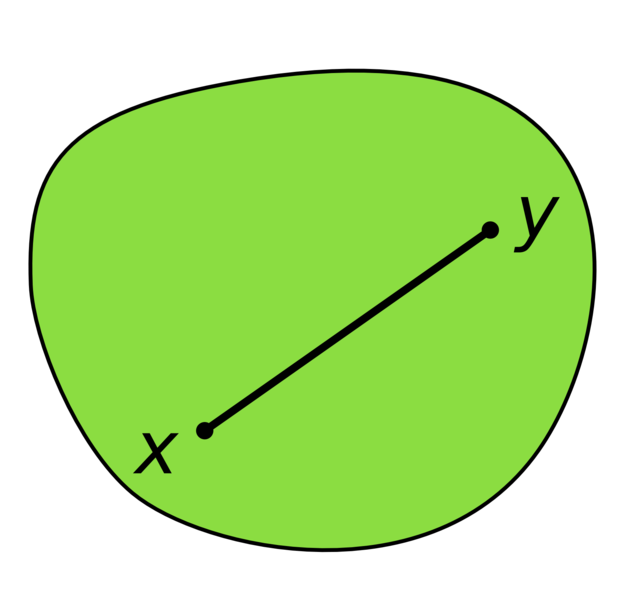
\includegraphics[width=0.30\textwidth]{img/convex2.png}}
\hspace{5mm}
\subfloat[Non convesso]
  {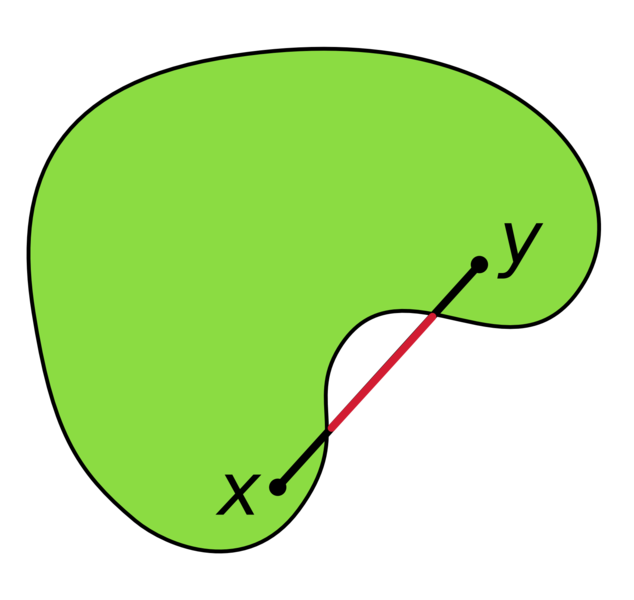
\includegraphics[width=0.30\textwidth]{img/convex1.png}}
\caption{Esempio di insiemi}
\label{convessi}
\end{figure}

\begin{definizione}[Convex Hull]
 Dato un insieme di punti, si dice \textbf{convex hull} (chiusura convessa) il più piccolo insieme convesso che li contiene tutti.
\end{definizione}

Il convex hull si può ottenere congiungendo con dei segmenti, i punti più ``esterni'' dell'insieme. Il convex hull di due punti sarà 
quindi il segmento che li congiunge. In figura \ref{fig:convexhull} è riportato il convex hull di 3 punti $p_1,p_2,p_3$. In generale, con k punti:
\begin{equation}
 CH(p_1,p_2,...,p_k)=\{ p \in R^n \mid p=\sum_{i=1}^k \lambda_i p_i \ \forall \bar{\lambda}=(\lambda_1,\lambda_2,...,\lambda_k) 
\in \Delta_k\}
\label{convex}
\end{equation}

\begin{figure}[htbp]
\begin{center}
	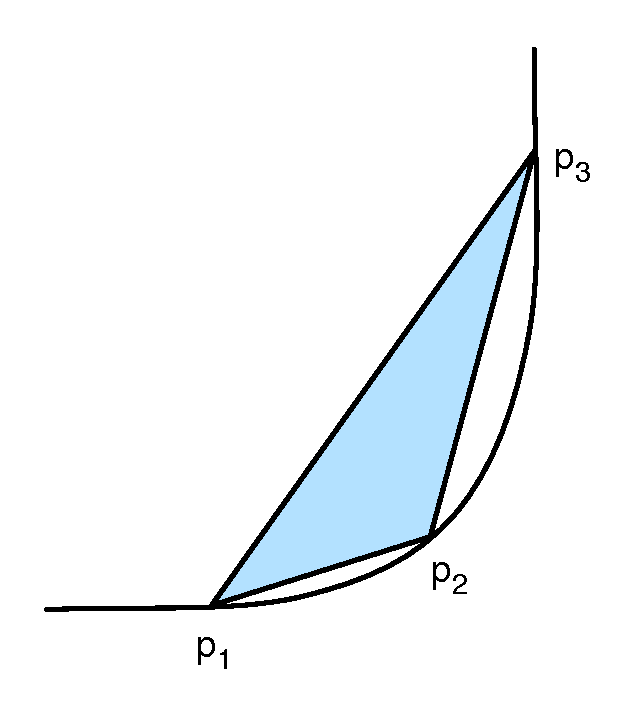
\includegraphics[width=0.35\textwidth]{img/convexhull.pdf}
\caption{Convex hull di $p_1,p_2,p_3$}
\label{fig:convexhull}
\end{center}
\end{figure}

Dalla definizione di funzione convessa e di convex hull, si può ricavare che data una funzione f convessa e comunque presi k punti $p_1,p_2,..p_k$ su y=f(x), risulta che $CH(p_1,p_2,...p_k)$ sta ``sopra`` y=f(x). L'esempio in figura \ref{fig:convexhull} mostra esattamente questo fatto con 3 punti (f è la curva).
Questo risultato è noto come disuguaglianza di Jensen. Tuttavia per arrivare alla forma ''finale`` della disuguaglianza, è necessario effettuare qualche passaggio a partire dall'idea che è stata appena esposta.

Potremo allora descrivere tutti gli infiniti punti del convex hull. Ovvero, data $f: [a,b] \to R$ convessa e comunque presi k punti 
$p_1,p_2,..p_k$ su y=f(x), risulta che:
\[
f(x) \le y, \forall P=(x,y) \in CH(p_1,p_2,...p_k)
\]
Stiamo in sostanza esprimendo il fatto che tutti i punti del convex hull stanno sopra la curva. Ma grazie alla \eqref{convex}, possiamo 
descrivere questi infiniti punti. Risulta dunque che:
\[
 P(x,y)=P \left (\sum_{i=1}^k \lambda_i x_i, \sum_{i=1}^k \lambda_i f(x_i) \right)  
                 \forall \bar{\lambda}=(\lambda_1,\lambda_2,...,\lambda_k) \in \Delta_k
\]

Possiamo ora arrivare alla versione finale della disuguaglianza.

\bigskip

\begin{teorema}[Disuguaglianza di Jensen]
 Sia $f: [a,b] \to R$ una funzione convessa, $x_1..x_k \in$ [a,b], $\bar{\lambda}=(\lambda_1,\lambda_2,...,\lambda_k) \in \Delta_k$.
 Allora vale che:
 \[
 f \left( \sum_{i=1}^k \lambda_i x_i \right) \le \sum_{i=1}^k \lambda_i f(x_i)
 \]
\begin{proof}
 Per prima cosa è necessario dimostrare che il teorema sia ''ben posto``, ovvero che f sia calcolata sempre 
 all'interno del dominio [a,b].
 Bisogna in sostanza dimostrare che:
 \[
  a \le x_i \le b  \ \ \forall i=1..k
 \]
 E che:
 \[
  a \le \sum_{i=1}^k \lambda_i x_i \le b \ \ \forall i=1..k
 \]

 \noindent
 Il primo caso è banale, infatti $x_1..x_k \in$ [a,b] per ipotesi.
 Per quanto riguarda il secondo caso invece osserviamo che $\lambda_i \ge0$ per ipotesi.
 Abbiamo quindi che:
 \[\begin{split}
  & a \le x_1 \le b \\
  \Rightarrow & \lambda_i a \le \lambda_i x_i \le \lambda_i b \\
  \Rightarrow & \sum_{i=1}^k \lambda_i a \le \sum_{i=1}^k \lambda_i x_i \le \sum_{i=1}^k \lambda_i b \\
  \Rightarrow & a \sum_{i=1}^k \lambda_i \le \sum_{i=1}^k \lambda_i x_i \le b \sum_{i=1}^k \lambda_i \\
  \Rightarrow & a \le \sum_{i=1}^k \lambda_i x_i \le b \\
   \end{split}
 \]
Il teorema è dunque ben posto. Possiamo allora iniziare la dimostrazione, per induzione su k (numero di punti).

\begin{description}
 \item[Caso base, k=2]
  \mbox{}

  Dobbiamo dimostrare che per ogni $\lambda_1,\lambda_2$ positivi, tali che $\lambda_1+\lambda_2=1$:
  \[
   f( \lambda_1 x_1 + \lambda_2 x_2) \le \lambda_1 f(x_1) + \lambda_2 f(x_2)
  \]
  Ma ciò è equivalente a:
  \[
   f( \lambda_1 x_1 + (1-\lambda_1) x_2) \le \lambda_1 f(x_1) + (1-\lambda_1) f(x_2)
  \]
  Che è banalmente vero, data la convessità di f.

 \item[Passo induttivo]
\mbox{}

Supponiamo che la disuguaglianza sia vera per k e dimostriamo che vale anche per k+1.
Pongo:
\[
 \mu_i=\frac{\lambda_i}{1-\lambda_{k+1}} \ i=1..k
\]
Osservo che $\mu_i>0 \forall i=1..k$ (rapporto di quantità positive) e che vale:
\[\begin{split}
 & \sum_{i=1}^k \mu_i=\sum_{i=1}^k \frac{\lambda_i}{1-\lambda_{k+1}} \\
 &= \frac{1}{1-\lambda_{k+1}} \sum_{i=1}^k \lambda_i
 = \frac{1-\lambda_{k+1}}{1-\lambda_{k+1}}=1
 \end{split}
\]
Considero ora la parte sinistra della disuguaglianza da dimostrare:
\[\begin{split}
 & f \left( \sum_{i=1}^{k+1} \lambda_i x_i \right) \\
 = & f \left( \sum_{i=1}^k \lambda_i x_i +\lambda_{k+1}x_{k+1} \right) \\
 = & f \left( \sum_{i=1}^k (1-\lambda_{k+1}) \mu_i x_i +\lambda_{k+1}x_{k+1} \right) \\
 = & f \left( (1-\lambda_{k+1}) \sum_{i=1}^k \mu_i x_i +\lambda_{k+1}x_{k+1} \right) \\
 \end{split}
\]

Ma poiché f è convessa (primo passaggio) e vale l'ipotesi induttiva (secondo passaggio):
\[\begin{split}
 & f \left( (1-\lambda_{k+1}) \sum_{i=1}^k \mu_i x_i +\lambda_{k+1}x_{k+1} \right) \\
 & \le (1-\lambda_{k+1})  f \left( \sum_{i=1}^k \mu_i x_i\right) +\lambda_{k+1} f(x_{k+1})  \\
 & \le (1-\lambda_{k+1})  \sum_{i=1}^k \mu_i f(x_i) +\lambda_{k+1} f(x_{k+1})  \\
 & = \sum_{i=1}^k \lambda_i f(x_i) +\lambda_{k+1} f(x_{k+1}) \\
 &= \sum_{i=1}^{k+1} \lambda_i f(x_i) \\
 \end{split}
\]

Riassumendo dunque abbiamo che:
\[
f \left( \sum_{i=1}^{k+1} \lambda_i x_i \right) \le \sum_{i=1}^{k+1} \lambda_i f(x_i)
\]

che dimostra il passo induttivo, concludendo la dimostrazione.
\end{description}
\end{proof}
\label{jensen}
\end{teorema}

\begin{corollario}
 Se inoltre f è strettamente convessa, vale che:
 \[
 f \left( \sum_{i=1}^k \lambda_i x_i \right) = \sum_{i=1}^k \lambda_i f(x_i) \iff \forall i \in \sigma(\bar{\lambda}) \ : \ x_i=const
 \]
 Dove $\sigma(\bar{\lambda})$ è detto supporto di $\bar{\lambda}$. Ovvero è l'insieme degli indici i per cui $\lambda_i \ne 0$
 \begin{proof}
 \mbox{}

  \begin{description}
   \item[\(\Longrightarrow\)] (Omesso, la dimostrazione è complicata)
   \item[\(\Longleftarrow\)] 
   Si ha che:
   \[\begin{split}
    & f \left( \sum_{i=1}^k \lambda_i x_i \right)=
    f \left( \sum_{i \in \sigma(\bar{\lambda}) } \lambda_i x_i \right) \\
    =& f \left( \sum_{i \in \sigma(\bar{\lambda}) } \lambda_i const \right)=
     f \left( const \sum_{i \in \sigma(\bar{\lambda}) } \lambda_i \right) \\
    =& f \left( const \right)= \sum_{i \in \sigma(\bar{\lambda}) } [\lambda_i] f \left( const \right) \\
    =& \sum_{i \in \sigma(\bar{\lambda}) } [\lambda_i f \left( const \right)] \\
    =& \left( \sum_{i=1}^k \lambda_i f(x_i) \right)
     \end{split}
   \]

  \end{description}
 \end{proof}
\end{corollario}

\bigskip

\noindent
Introduciamo ora il concetto di metrica (o distanza), al fine di descrivere una particolare distanza.

\begin{definizione}[Metrica]
 Dato un insieme X, una metrica (o distanza) è una funzione
\[
 d: X \times X \to R
\]
Per cui valgono le seguenti proprietà, $\forall x,y,z \in X$:
\[\begin{split}
 & 1) d(x,y) \ge 0 \\
 & 2) d(x,y)=0 \iff x=y \\
 & 3) d(x,y)=d(y,x) \\
 & 4) d(x,y) \le d(x,z)+d(z,y)
 \end{split}
\]
\end{definizione}

\begin{definizione}[Distanza di Kullback-Leibler]
\mbox{}

 Dati $\bar{p} \ e \ \bar{q} \in \Delta_n$, la lora distanza di Kullback-Leibler è:
\[
 D_{KL}(\bar{p} \| \bar{q})=\sum_{i=1}^n p_i log\frac{p_i}{q_i}
\]

(Assumiamo che $0 log0=0$ e $p_i log \frac{p_i}{0}=\infty$ )
\label{distkl}
\end{definizione}

\begin{osservazione}
 La distanza di Kullback-Leibler non è una metrica. Non valgono infatti le proprietà 3 e 4.
\end{osservazione}

\begin{teorema}
 La distanza di Kullback-Leibler soddisfa le proprietà 1 e 2 di metrica.
 Ovvero, date $\bar{p}$ e $\bar{q} \in \Delta_n$ (distribuzioni di probabilità):

 \begin{itemize}
  \item[(i)]  $D_{KL}(\bar{p} \| \bar{q}) \ge 0$
  \item[(ii)] $D_{KL}(\bar{p} \| \bar{q}) = 0 \iff \bar{p}=\bar{q}$
 \end{itemize}

\begin{proof}
 \mbox{}

 \begin{description}
 \item[(i)]
  \[\begin{split}
    &-D_{KL}(\bar{p} \| \bar{q})= -\sum_{i=1}^n p_i log \frac{p_i}{q_i} \\
    &=\sum_{i=1}^n p_i log \frac{q_i}{p_i} \\
    &=\sum_{i \in \sigma(\bar{p})} p_i log \frac{q_i}{p_i} \\
    \end{split}
  \]
  Ora posso applicare la disuguaglianza di Jensen (teorema \ref{jensen}). Tuttavia 
  il verso della disuguaglianza sarà inverso, in quanto la funzione logaritmo è concava e non convessa.
 \[\begin{split}
  &\sum_{i \in \sigma(\bar{p})} p_i log \frac{q_i}{p_i} \\
   \le & log \sum_{i \in \sigma(\bar{p})} p_i \frac{q_i}{p_i} \\
  =& log \sum_{i \in \sigma(\bar{p})} q_i \\
  \le & log \sum_{i=1}^n q_i \\
  =& log 1=0
  \end{split}
 \]

  Abbiamo quindi dimostrato che:
  \[
   -D_{KL}(\bar{p} \| \bar{q}) \le 0
  \]
  Da cui:
  \[
   D_{KL}(\bar{p} \| \bar{q}) \ge 0
  \]
 \item[(ii)]
  Possiamo utilizzare quanto dimostrato nel punto (i). In particolare, la distanza sarà zero se e solo se 
  le due disuguaglianze che compaiono sono uguaglianze.
  Per quanto riguarda la seconda disuguaglianza:
  \[\begin{split}
   &log \sum_{i \in \sigma(\bar{p})} q_i=log \sum_{i=1}^n q_i \\
   \iff &\sum_{i \in \sigma(\bar{p})} q_i=\sum_{i=1}^n q_i \\
   \iff & \forall i \notin \sigma(\bar{p}) : p_i=q_i
   \end{split}
  \]
   Ciò è vero in quanto, affinché i due termini coincidano, al di fuori del supporto di p non devono esserci indici i per cui 
   $q_i \ne 0$ (altrimenti la sommatoria ''completa`` sarebbe più grande ristretto a quella limitata al supporto di p).
   Ma se i non appartiene al supporto di p, allora $p_i=0$. Pertanto deve essere $p_i=q_i=0$, per $i \notin \sigma(\bar{p})$.

   Per quanto riguarda invece la prima disuguaglianza, si avrà uguaglianza solamente nel caso limite dato dal corollario al teorema 
   di Jensen (si noti che la funzione logaritmo è strettamente concava).
   Per il corollario bisogna avere che:
   \[
    \forall i \in \sigma(\bar{\lambda}) \ : \ x_i=const
   \]
   Nel caso in esame dunque:
   \[
    \forall i \in \sigma(\bar{p}) \ : \ \frac{q_i}{p_i}=const
   \]
   Quindi:
   \[
    \forall i \in \sigma(\bar{p}) \ : q_i=const \ p_i
   \]

   Da cui:
   \[ \begin{split}
    \sum_{i \in \sigma(p)} q_i &=\sum_{i \in \sigma(p)} const \ p_i \\
     &=const \sum_{i \in \sigma(p)} p_i \\
     &=const=1
    \end{split}
   \]
   Quindi deve essere const=1, ovvero:
   \[
    \forall i \in \sigma(\bar{p}) \ : p_i=q_i
   \]
   Riassumendo quindi le due condizioni si ha uguaglianza se e solo se:
   \[
    \forall i=1..n : p_i=q_i \ \ \iff \ \ \bar{p}=\bar{q}
   \]

\end{description}

\end{proof}
\label{leibler}
\end{teorema}

La distanza di Kullback-Leibler è anche nota come \textit{entropia relativa} e misura in un certo senso la distanza tra due distribuzioni di probabilità. Vediamo ora il concetto, molto importante, di informazione mutua (che è una particolare distanza di Kullback-Leibler).

\begin{definizione}[Informazione mutua]
 Date X,Y v.a e posto al solito $p(x)=Pr\{X=x\}$, $p(y)=Pr\{Y=y\}$, $p(x,y)=Pr\{X=x, Y=y\}$ si definisce 
 informazione mutua:
 \[
  I(X;Y)=\sum_{x \in X} \sum_{y \in Y} p(x,y) log \frac{p(x,y)}{p(x)p(y)}
 \]
\end{definizione}

\begin{osservazione}
 L'informazione mutua è una specifica distanza di Kullback-Leibler: $D_{KL}(p(x,y) \|  p(x)p(y))$.
 \begin{proof}
  Bisogna innanzitutto verificare che p(x)p(y) sia una distribuzione di probabilità.
  In maniera banale (prodotto di due probabilità):
  \[
   0 \le p(x)p(y) \le 1 \ \ \forall x \in X,y \in Y
  \]
  Risulta poi:
  \[\begin{split}
   &\sum_{x \in X}\sum_{y \in Y} p(x)p(y) \\
   =&\sum_{x \in X} p(x) \sum_{y \in Y}p(y) \\
   =& 1 \times 1 \\
   =&1 
    \end{split}
  \]
  p(x)p(y) è dunque una distribuzione di probabilità.
  Ponendo $p_i=p(x,y)$ e $q_i=p(x)p(y)$, si ottiene la distanza KL.
 \end{proof}

\end{osservazione}

In sostanza quindi, l'informazione mutua misura in un certo senso il grado di dipendenza tra due v.a.
Se infatti le due variabili sono indipendenti, allora p(x,y)=p(x)p(y) e quindi l'informazione mutua vale zero. Viceversa, più le 
variabili sono dipendenti tra loro, più la distanza aumenta. Vediamo ora come l'informazione mutua sia strettamente legata 
al concetto di entropia.

\begin{teorema}
\[
 I(X;Y)=H(X)-H(X/Y)=H(Y)-H(Y/X)
\]
\begin{proof}
\[\begin{split}
 I(X;Y)=&\sum_{x \in X} \sum_{y \in Y} p(x,y) log \frac{p(x,y)}{p(x)p(y)} \\
   =&\sum_{x \in X} \sum_{y \in Y} p(x,y) log \frac{p(y)p(x/y)}{p(x)p(y)} \\
   =&\sum_{x \in X} \sum_{y \in Y} p(x,y) log \frac{p(x/y)}{p(x)} \\
   =&\sum_{x \in X} \sum_{y \in Y} p(x,y) log (p(x/y))-\sum_{x \in X} \sum_{y \in Y} p(x,y) log (p(x)) \\
   =&-H(X/Y)-\sum_{x \in X} log (p(x)) \sum_{y \in Y} p(x,y)\\
   =&-H(X/Y)-\sum_{x \in X} log (p(x)) p(x)\\
   =&-H(X/Y)+H(X)\\
   =&H(X)-H(X/Y)\\
 \end{split}
\]
In maniera del tutto analoga si dimostra la seconda uguaglianza.
\end{proof}
\label{infmutua}
\end{teorema}

In sostanza quindi l'informazione mutua può anche essere vista come differenza di entropie. Utilizzando, ad esempio, la prima 
uguaglianza l'informazione mutua tra X e Y mi dice l'incertezza che mi rimane sulla variabile X, dopo aver ''conosciuto`` la variabile 
Y. Come si vedrà più avanti, questo fatto costituisce la base per l'analisi dei canali di trasmissione (nello specifico è fondamentale 
per calcolare la capacità di un canale).

\begin{osservazione}
 I(X;Y)=H(X)+H(Y)-H(X,Y)
 \begin{proof}
  Per il teorema \ref{infmutua}:
  \[
  I(X;Y)=H(X)-H(X/Y)
  \]
  Per la regola della catena (Teorema \ref{catena}):
  \[\begin{split}
  I(X;Y)&=H(X)-[H(X,Y)-H(Y)] \\
        &=H(X)+H(Y)-H(X,Y)
    \end{split}
  \]
 \end{proof}
\end{osservazione}

Si può utilizzare un diagramma di Venn, per rappresentare (in maniera intuitiva) la relazione tra entropia ed informazione mutua (Figura \ref{fig:mutua}).

\begin{figure}[htbp]
\begin{center}
	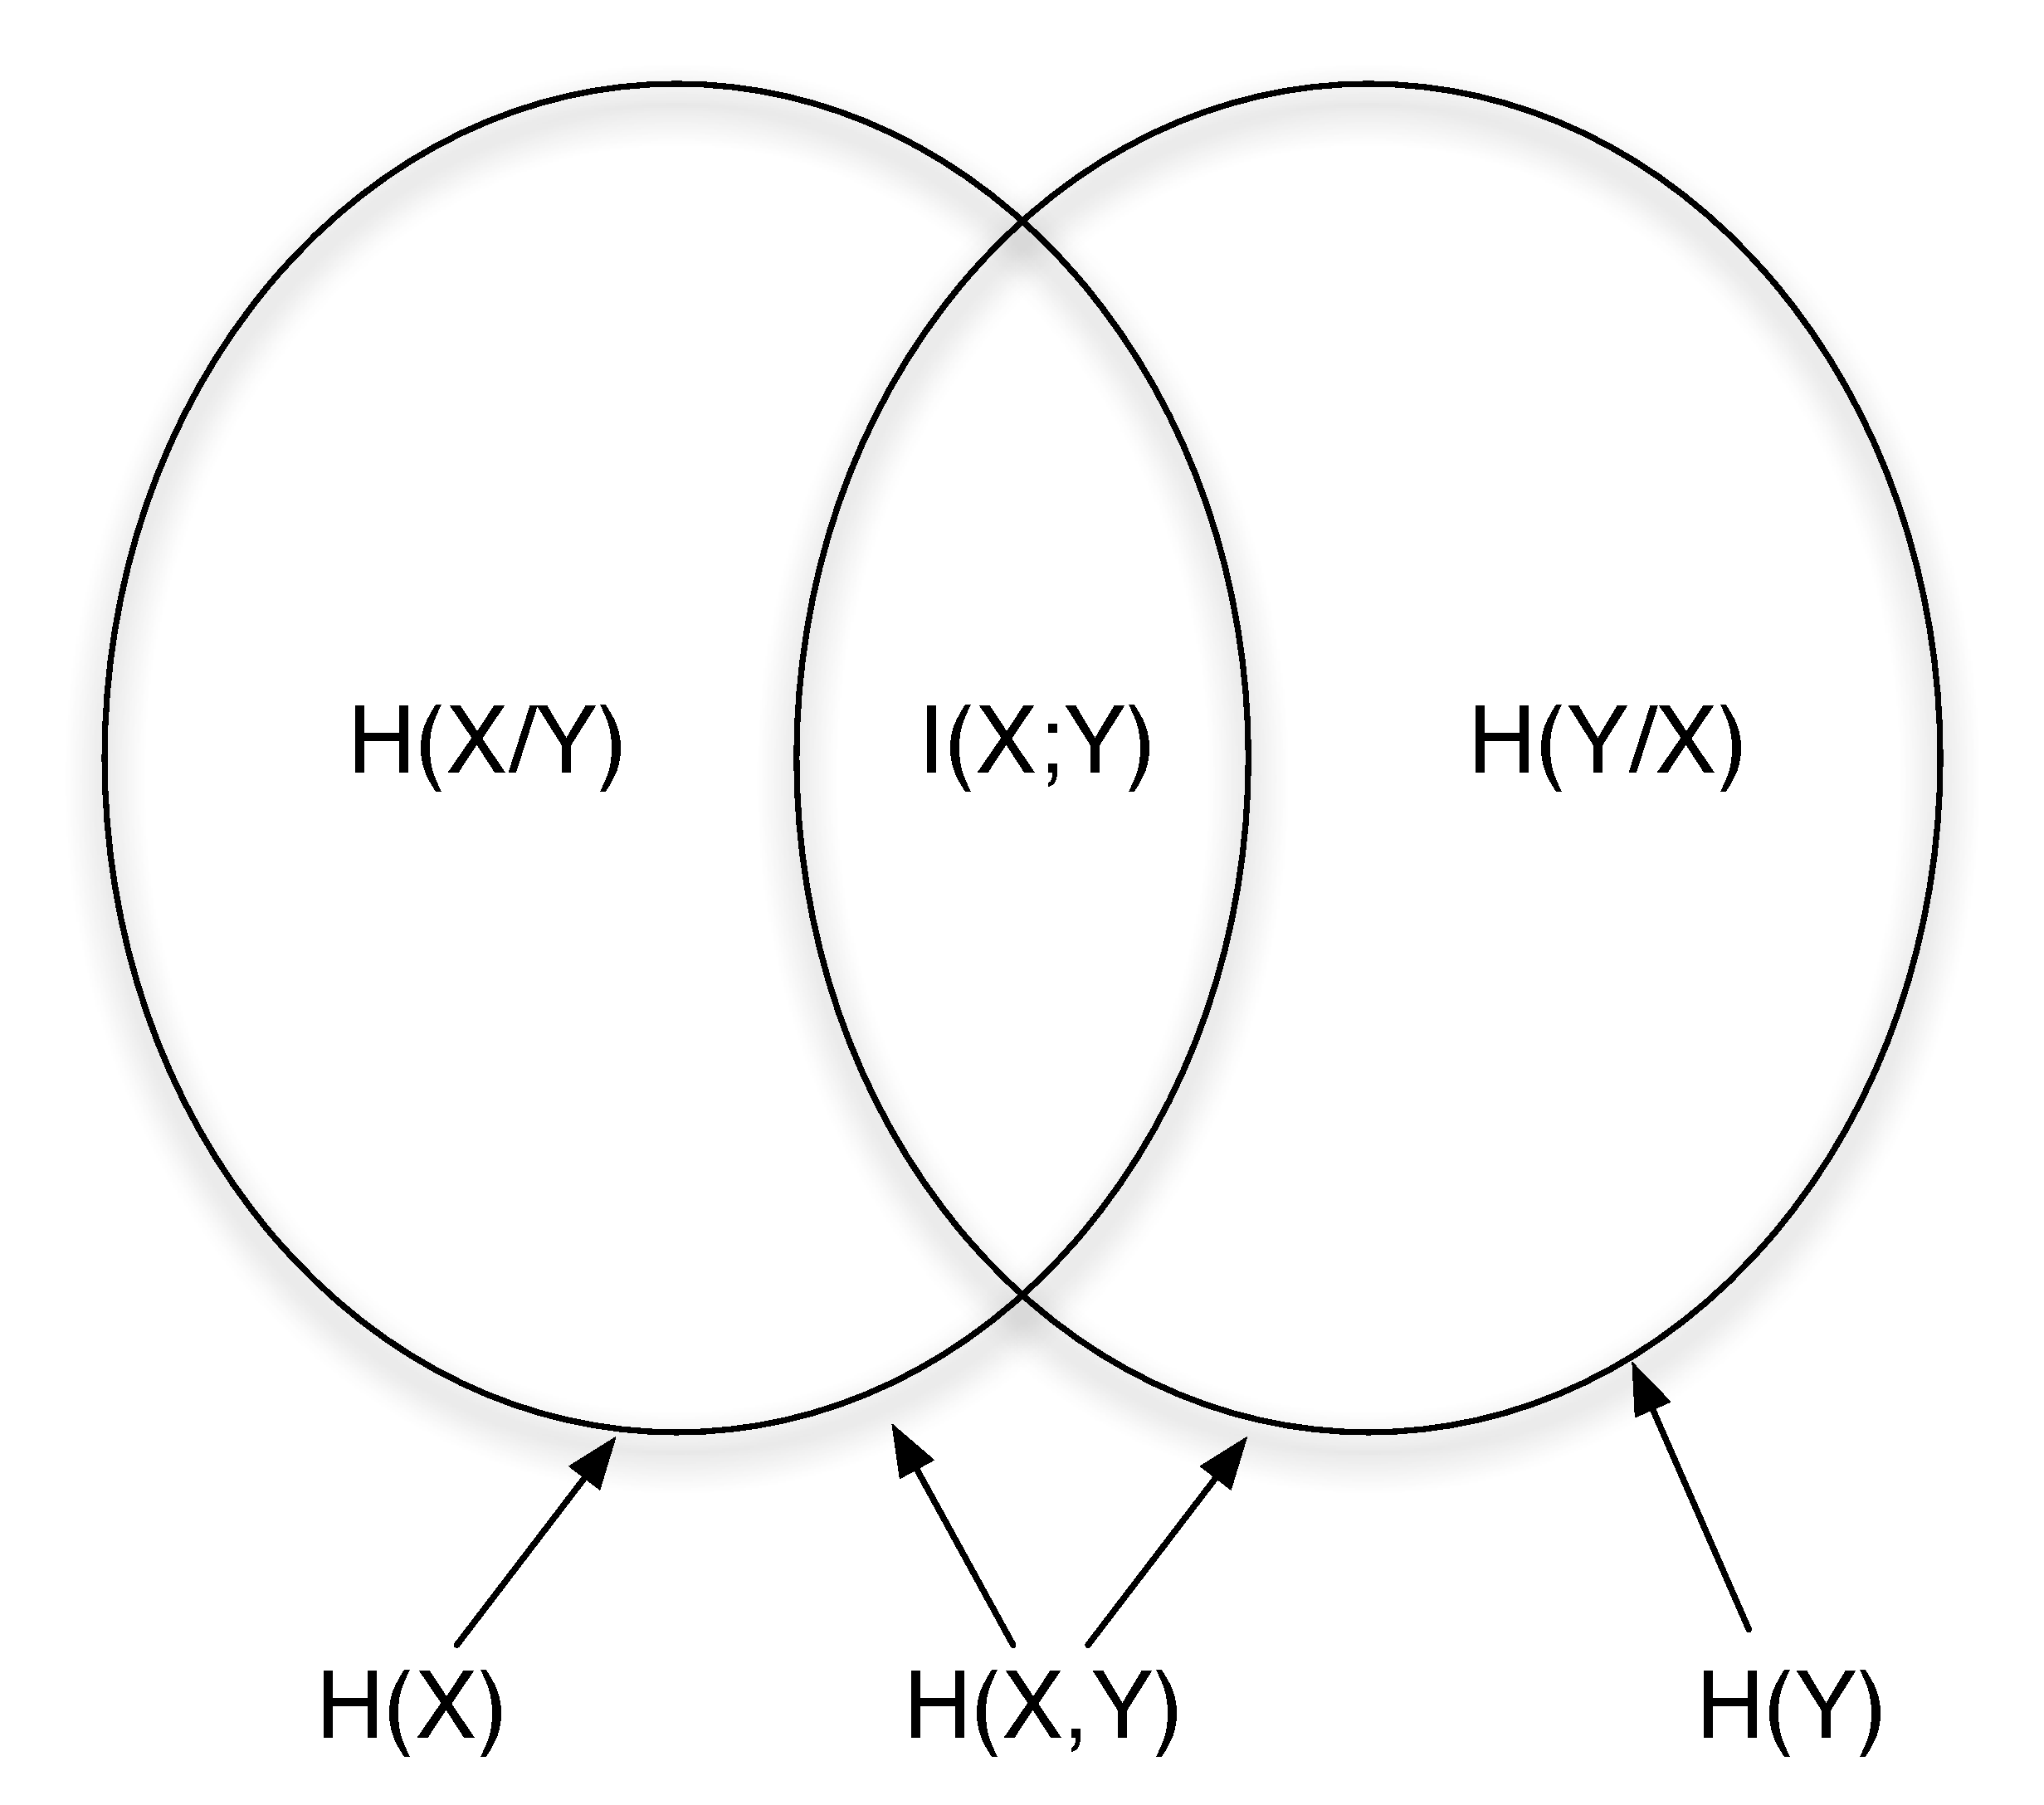
\includegraphics[width=0.5\textwidth]{img/mutua.pdf}
\caption{Relazione tra entropia ed informazione mutua}
\label{fig:mutua}
\end{center}
\end{figure}

\noindent
Possiamo, sempre sulla base del teorema \ref{infmutua}, effettuare una serie di osservazioni sull'informazione mutua.

\begin{osservazione}
\[
 I(X;X)=H(X)
\]
\end{osservazione}

\begin{osservazione}
 \[
   I(X;Y) \ge 0  
 \]
 \begin{proof}
  Banale, poiché l'informazione mutua è una distanza KL che è maggiore o uguale a 0 per il teorema \ref{leibler}.
 \end{proof}
\label{distinf}
\end{osservazione}

\begin{osservazione}
 \[
   I(X;Y)=0 \iff X \ e \ Y \ sono \ statisticamente \ indipendenti  
 \]
 \begin{proof}
  Per il teorema \ref{leibler} una distanza KL è 0 se e solo se le due distribuzioni di probabilità coincidono.
  In questo caso quindi, se e solo se p(x,y)=p(x)p(y) (che è proprio la definizione di indipendenza).
 \end{proof}
 \label{mutuaindip}
\end{osservazione}

\begin{osservazione}[Il condizionamento riduce l'entropia]
 \[
  H(X/Y) \le H(X)
 \]
  \begin{proof}
   \[\begin{split}
     & H(X/Y) \le H(X) \\ 
     \iff & H(X/Y) -H(X) \le 0 \\
     \iff & H(X)-H(X/Y) \ge 0 \\
     \iff & I(X;Y) \ge 0
     \end{split}
   \]
  Ma per l'osservazione \ref{distinf}, l'informazione mutua è sempre maggiore o uguale a zero.
  \end{proof}

 \label{condizionamento}
\end{osservazione}

\begin{osservazione}
 La funzione entropia è concava. Ovvero dati:
 \[
 \bar{p} \in \Delta_n \\
 H(\bar{p})=-\sum_{i=1}^n p_i log(p_i)
 \]
 Vale che:
 \[
  \forall \lambda \in [0,1] \ e \ \bar{p}_1,\bar{p}_2 \in \Delta_n \ : \ 
   H(\lambda \bar{p}_1 + (1-\lambda) \bar{p}_2) \ge \lambda H(\bar{p}_1) + (1-\lambda) H(\bar{p}_2)
 \]

\begin{proof}
 Consideriamo $\X=\{1..n\}$ e costruiamo due variabili casuali $X_1,X_2$ con valori in $\X$, così distribuite:
 \[
  X_1 \sim \bar{p_1} \\ X_2 \sim \bar{p_2}
 \]
 Consideriamo poi una variabile $\Theta$ nell'insime $\{1,2\}$, così distribuita:
 \[
  Pr\{\Theta=1\}=\lambda \\ Pr\{\Theta=2\}=1-\lambda
 \]
 Costruiamo infine una variabile Z che varia nell'insieme X, definita come:
 \[
  Z=X_{\Theta}
 \]
 In altre parole Z è una variabile composta, che vale $X_1$ con probabilità $\lambda$ e $X_2$ con probabilità $1-\lambda$.
 Ora analizziamo la distribuzione Z, calcolando $Pr\{Z=x\} , \ x \in X$:
 \[\begin{split}
  Pr\{Z=x\}=&Pr\{[\Theta=1 \land X_1=x] \lor [\Theta=2 \land X_2=x]  \} \\
  =&Pr\{[\Theta=1 \land X_1=x]\} + Pr\{[\Theta=2 \land X_2=x]  \} \\
  =&Pr\{\Theta=1\} Pr\{X_1=x\} + Pr\{\Theta=2\} Pr\{X_2=x\} \\
  =& \lambda \bar{p}_{1x} + (1-\lambda) \bar{p}_{2x}
  \end{split}
 \]
  Dove con $\bar{p}_{1x}$ abbiamo indicato la componente x° di $\bar{p}_1$ (similmente per $\bar{p}_2$).
  Risulta quindi che:
  \[
   Z \sim q=\lambda \bar{p}_1 + (1-\lambda) \bar{p}_2
  \]
  Da cui:
  \[
   H(Z)=H(\lambda \bar{p}_1 + (1-\lambda) \bar{p}_2)
  \]
  Ora semplifichiamo $H(Z/\Theta)$. Risulta:
  \[\begin{split}
   H(Z/\Theta)=&Pr\{\Theta=1\}H(Z/\Theta=1)+Pr\{\Theta=2\}H(Z/\Theta=2) \\
   =& \lambda H(Z/\Theta=1)+(1-\lambda)H(Z/\Theta=2) \\
   =& \lambda H(X_1)+(1-\lambda)H(X_2) \\
   =& \lambda H(\bar{p}_1)+(1-\lambda)H(\bar{p}_2) \\
   \end{split}
  \]
  Riassumendo si ha dunque che:
  \[
    H(Z)=H(\lambda \bar{p}_1 + (1-\lambda) \bar{p}_2) \\ H(Z/\Theta)=\lambda H(\bar{p}_1)+(1-\lambda)H(\bar{p}_2)
  \]
  Ora, per l'osservazione \ref{condizionamento} il condizionamento riduce l'entropia. Vale quindi:
   \[
     H(Z/\Theta) \le H(Z) 
  \]
  Ovvero:
  \[\begin{split}
   & H(Z/\Theta) \le H(Z) \\
   \iff & H(Z) \ge H(Z/\Theta)  \\
   \iff &  H(\lambda \bar{p}_1 + (1-\lambda) \bar{p}_2) \ge \lambda H(\bar{p}_1)+(1-\lambda)H(\bar{p}_2)
   \end{split}
  \]


\end{proof}
\label{entrconcava}
\end{osservazione}

In maniera analoga a quanto fatto per l'entropia, cerchiamo ora di definere l'informazione mutua condizionata.
Vogliamo in sostanza calcolare:
\[
 I(X,Y/Z)
\]
Al solito, calcoliamo prima il valore per uno specifico $z \in Z$:
\[\begin{split}
 I(X,Y/Z=z)&=D_{KL}[p(x,y/z) \ \| \ p(x/z)p(y/z)] \\
 &=\sum_{x \in X} \sum_{y \in Y} p(x,y/z) log \frac{p(x,y/z)}{p(x/z)p(y/z)}
  \end{split}
\]

\noindent
Calcoliamo poi (sempre come già fatto per l'entropia) il valore atteso rispetto a Z:
\[
 \begin{split}
 I(X,Y/Z)&=\sum_{z \in Z} p(z) I(X,Y/Z=z) \\
 &=\sum_{z \in Z} \sum_{x \in X} \sum_{y \in Y} p(z)p(x,y/z) log \frac{p(x,y/z)}{p(x/z)p(y/z)} \\
 &=\sum_{z \in Z} \sum_{x \in X} \sum_{y \in Y} p(x,y,z) log \frac{p(x,y/z)}{p(x/z)p(y/z)}
  \end{split}
\]

\bigskip
\noindent
Naturalmente non siamo in presenza di una forma ''compatta``. Tuttavia a partire da questo risultato, 
si può arrivare alla seguente osservazione.

\begin{osservazione}
 \[
 I(X,Y/Z)=H(X/Z)-H(X/Y,Z)
\]
\end{osservazione}

\begin{osservazione}
 \[
  I(X,Y/Z) \ge 0
 \]
\end{osservazione}

\begin{osservazione}
\[
 H(X_1,X_2,..,X_n)=\sum_{i=1}^n H(X_i/X_1,X_2,..X_{i-1}) \le \sum_{i=1}^n H(X_i)
\]
\end{osservazione}


\section{Asymptotic Equipartition Property}
\label{aep}
La AEP (Asymptotic Equipartition Property) è la variante della legge dei grandi numeri, nel campo della teoria dell'informazione.
La legge (debole) dei grandi numeri, importante risultato nel campo della statistica, può essere riassunta nel modo seguente.

Siano $Z_1..Z_n$ delle variabili aleatorie i.i.d (indipendenti e identicamente distribuite) ciascuna con media $\mu$ e varianza $\sigma^2$.
Sia inoltre $\bar{Z}_n$ la media campionaria di queste n variabili, ovvero:
\[
 \bar{Z}_n=\frac{1}{n} \sum_{i=1}^n Z_i
\]

Allora vale che:
\[
 \forall \epsilon > 0: \\
 \lim_{n\to\infty}Pr(|\bar{Z}_n-\mu|\le \epsilon)=1
\]

Possiamo in sostanza dire che (per n grande) la media campionaria tende in probabilità al valore atteso.

Siano ora $X_1..X_n$ delle variabili aleatorie i.i.d. Indichiamo con $X^n$ l'insieme di tutte le sequenze possibili e con $\bar{x}=(x_1,x_2,...x_n) \in X^n $ una generica sequenza.

\bigskip
\noindent
\textbf{Esempio}

\noindent
Siano $A_1$ e $A_2$ due v.a. i.i.d, definite nell'insieme $\{1,2,3\}$.
Allora:
\[
 A^2=\Bigl \lbrace \{1,1\},\{1,2\},\{1,3\},\{2,1\},\{2,2\},\{2,3\},\{3,1\},\{3,2\},\{3,3\} \Bigl \rbrace
\]
Una generica sequenza $\bar{a}$ è (ad esempio) $\{2,3\}$.

\bigskip
Possiamo dividere l'insieme $X^n$ in due parti: l'insieme delle sequenze tipiche e l'insieme delle sequenza atipiche.

\begin{definizione}
 L'insieme delle sequenze ($\epsilon$,n)-tipiche è:
\[
 A_{\epsilon}^n=\{ \bar{x} \in X^n \mid 2^{-n(H(x)+\epsilon)} \le p(\bar{x}) \le 2^{-n(H(x)-\epsilon)} \}
\]
\label{tipiche}
\end{definizione}

\noindent
Stiamo in sostanza affermando che le sequenze tipiche hanno tutte circa la stessa probabilità: 
$p(\bar{x}) \backsimeq 2^{-nH(x)} \ \forall \bar{x} \in A_{\epsilon}^n$

\begin{teorema}[AEP]
 \[
  \lim_{n \to \infty} Pr\{A_{\epsilon}^n\}=1
 \]
 \begin{proof}
  \[
  \begin{split}
    \bar{x} \in A_{\epsilon}^n &\iff 2^{-n(H(x)+\epsilon)} \le p(\bar{x}) \le 2^{-n(H(x)-\epsilon)} \\
    &\iff -n(H(x)+\epsilon) \le log(p(\bar{x})) \le -n(H(x)-\epsilon) \\
    &\iff -(H(x)+\epsilon) \le \frac{1}{n} log(p(\bar{x})) \le -(H(x)-\epsilon) \\
    &\iff H(x)-\epsilon \le -\frac{1}{n} log(p(\bar{x})) \le H(x)+\epsilon \\
    &\iff \mid -\frac{1}{n} log(p(\bar{x})) - H(x) \mid \le \epsilon  \\
  \end{split}
  \]

 Consideriamo ora $Z_1..Z_n$ v.a. i.i.d e poniamo
 \[
  Z_i= -log( p(X_i) )
 \]
 
  \noindent
  Calcoliamo allora la media campionaria delle variabili Z:
  \[
  \begin{split}
   \bar{Z}_n &=\frac{1}{n} \sum_{i=1}^n Z_i \\
             &=\frac{1}{n} \sum_{i=1}^n -log(p(X_i)) \\
             &=-\frac{1}{n} log \left [ \prod_{i=1}^n (p(X_i) \right] \\
             &=-\frac{1}{n} log(p(\bar{x}))
  \end{split}
  \]
  L'ultimo passaggio è dovuto all'indipendenza delle variabili.
  Consideriamo ora il valore atteso delle variabili Z:
  \[
  \begin{split}
   \mu &=\sum_{i=1}^n p(Z_i) Z_i \\
        &=\sum_{i=1}^n p(X_i)(-log(p(X_i)) \\
             &=H(X)
  \end{split}
  \]
  Risulta quindi:
  \[ \begin{split}
   \bar{x} \in A_{\epsilon}^n &\iff \mid -\frac{1}{n} log(p(\bar{x})) - H(x) \mid \le \epsilon \\
   &\iff \mid \bar{Z}_n - \mu \mid \le \epsilon
    \end{split}
  \]
  Da cui, per la legge dei grandi numeri:
  \[
  \lim_{n \to \infty} Pr\{A_{\epsilon}^n\}=
     \lim_{n \to \infty} Pr\{ \mid \bar{Z}_n - \mu \mid \le \epsilon \}=1
 \]

 \end{proof}

\end{teorema}

Per chiarire meglio i concetti esposti, possiamo rappresentare graficamente l'insieme $X^n$ delle sequenze, che 
contiene quelle tipiche e quelle atipiche (figura \ref{fig:sequenze}).
Si nota come si tratti di due insiemi disgiunti. Il teorema AEP ci dice che, per n sufficientemente grande, la probabilità 
di avere una sequenze tipica tende a 1. Inoltre, tutte le sequenze tipiche sono circa equiprobabili.

\begin{figure}[htbp]
\begin{center}
	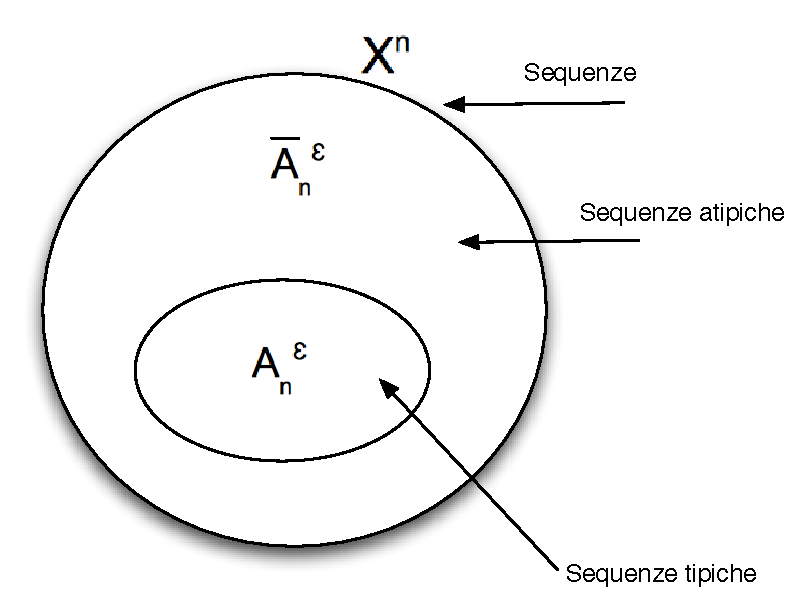
\includegraphics[width=0.6\textwidth]{img/sequenze.pdf}
\caption{Rappresentazione grafica delle sequenze}
\label{fig:sequenze}
\end{center}
\end{figure}

\bigskip
\noindent
\textbf{Esempio}

\noindent
Consideriamo il lancio di una moneta. Supponiamo di effettuare n lanci (con n grande) e costruire quindi sequenze lunghe n.
Se la moneta è totalmente sbilanciata ed esce sempre testa (probabilità di avere testa 1, di croce 0), allora ci sarà solo una sequenza
tipica: quella formata da tutte teste. Le altre sequenze infatti non potranno mai verificarsi.
Se la moneta è invece perfettamente bilanciata (probabilità di avere testa uguale a probabilità di avere croce) tutte le sequenze 
saranno tipiche. E' facile infatti notare che sono tutte equiprobabili.

\bigskip
E' interessante a questo punto sapere quanti elementi contiene l'insieme delle sequenze tipiche. Intuitivamente (per n suff. grande) la
sua cardinalità dovrebbe essere $2^{nH(x)}$. Infatti $1/2^{-nH(x)}=2^{nH(x)}$ poiché la probabilità totale è 1 e tutte le sequenze 
tipiche sono equiprobabili.

\bigskip
\noindent
\textbf{Esempio}

\noindent
Riprendiamo l'esempio della moneta considerato prima e proviamo a calcolare la cardinalità dell'insieme sequenze tipiche.
Per quanto detto il numero delle sequenze tipiche dovrebbe essere $2^{nH(x)}$.
Nel caso in cui la moneta è bilanciata, l'entropia risulta:
\[
 H(X)=H \left( \frac{1}{2},\frac{1}{2} \right)=1
\]
Quindi la cardinalità sarebbe $2^n$, ovvero tutte le sequenze sono tipiche (la cardinalità di $X^n$ è banalmente $2^n$).
Se consideriamo invece la moneta in cui la probabilità di avere testa è 1, allora l'entropia risulta:
\[
 H(X)=H \left(1\right)=0
\]
Quindi la cardinalità dovrebbe essere $2^{n0}=1$, ovvero esiste un'unica sequenza tipica.

\bigskip
Quanto detto finora è solo un ragionamento intuitivo, formalizziamo in maniera più accurata questo punto tramite alcune 
proposizioni.

\begin{osservazione}
 \[
   \forall \epsilon > 0, \ \exists n_0 \mid \forall n \ge n_0 \ : \ Pr\{A_{\epsilon}^n\} \ge 1 - \epsilon 
 \]
  
  \begin{proof}
   Una successione $\{a_n\}$ ha limite l $\in$ R se $\forall \delta > 0$: 
   \[
    \exists n_o \mid \forall n \ge n_0 : \ \mid a_n-l \mid \le \delta
   \]

   Ma per il teorema AEP:
   \[ \begin{split}
    & \lim_{n \to \infty} Pr\{A_{\epsilon}^n\}=1 \\
    & \Rightarrow \mid Pr\{A_{\epsilon}^n\} -1 \mid \le \delta \\
    & \Rightarrow 1- Pr\{A_{\epsilon}^n\} \le \delta \\
    & \Rightarrow Pr\{A_{\epsilon}^n\} \ge 1- \delta
    \end{split}
   \]
   Poniamo $\delta=\epsilon$ per concludere la dimostrazione.
  \end{proof}
\label{ossAep}
\end{osservazione}

\begin{proposizione}
 \mbox{}
 \begin{itemize}
  \item[(i)] $ |A_{\epsilon}^n| \le 2^{n(H(x)+\epsilon)}$
 
  \item[(ii)] $|A_{\epsilon}^n| \ge (1-\epsilon) 2^{n(H(x)-\epsilon)}$  (per n suff. grande)
 \end{itemize}
 \begin{proof}
  \mbox{}
  \begin{itemize}
   \item[(i)] Si ha che:
   \[
    1=\sum_{x \in X^n} p(x) \ge \sum_{x \in A_{\epsilon}^n} p(x) \ge 
      \sum_{x \in A_{\epsilon}^n} 2^{-n(H(x)+ \epsilon)}=|A_{\epsilon}^n| 2^{-n(H(x)+ \epsilon)} 
   \]
   Da cui:
   \[
    |A_{\epsilon}^n| 2^{-n(H(x)+ \epsilon)} \le 1 \Rightarrow |A_{\epsilon}^n| \le 2^{n(H(x)+ \epsilon)}
   \]


   \item[(ii)]
   Per l'osservazione \ref{ossAep}:
   \[
    \forall \epsilon > 0, \ \exists n_0 \mid \forall n \ge n_0 \ : \ 1 - \epsilon \le Pr\{A_{\epsilon}^n\}
   \]
   Da cui:
   \[
    1 - \epsilon \le Pr\{A_{\epsilon}^n\}=\sum_{x \in A_{\epsilon}} p(x) \le 
    \sum_{x \in A_{\epsilon}} 2^{-n(H(x)-\epsilon)} = |A_{\epsilon}^n| 2^{-n(H(x)-\epsilon)}
   \]
   Risulta quindi:
   \[\begin{split}
    & 1 - \epsilon \le |A_{\epsilon}^n| 2^{-n(H(x)-\epsilon)}  \\
    & \Rightarrow |A_{\epsilon}^n| 2^{-n(H(x)-\epsilon)}  \ge 1 - \epsilon \\
    &\Rightarrow |A_{\epsilon}^n| \ge (1 - \epsilon) 2^{n(H(x)-\epsilon)}
    \end{split}
   \]

  \end{itemize}

 \end{proof}

\end{proposizione}

Ques'ultima proposizione dimostra che la nostra intuizione era corretta e formalizza in maniera precisa all'interno 
di quali estremi si trova la cardinalità dell'insieme delle sequenze tipiche.

\subsection{Generalizzazione dell'AEP}

L'AEP fornisce dei risultati importanti, tuttavia ha delle ipotesi abbastanza restrittive. In particolare, abbiamo supposto che le v.a. 
$X_1..X_n$, fossero i.i.d. Nel caso di una sorgente generica, ciò equivale a dire che essa è senza memoria. Non sempre però è lecito fare questa assunzione. Per fare un esempio, se la sorgente emette delle lettere che costituiscono parole in lingua italiana, dopo la lettera e.g. h, seguirà con tutta probabilità una vocale. In questo contesto quindi non si potrebbe accettare l'ipotesi di indipendenza e non si potrebbe dunque applicare l'AEP.

Mettiamoci dunque in un caso più generale, considerando un processo stocastico. Possiamo pensare ad un processo stocastico, come ad una famiglia di variabili casuali $X_1..X_n$. Indicheremo tale processo nel seguente modo:
\[
 \{X_t\}_{t=1..\infty}
\]

In questo contesto possiamo pensare al processo come ad una sorgente, che genera appunto $X_1..X_n$. Ora, a seconda delle relazioni 
tra le variabili, possiamo avere diversi tipi di processi. Consideriamo i seguenti casi:
\begin{itemize}
 \item $X_1..X_n$ i.i.d. E' il caso che abbiamo considerato fino ad ora, in cui le variabili sono indipendenti
 \item Catena di Markov: E' un processo stocastico, per cui vale la seguente proprietà:
  \[\begin{split}
   &Pr\{ X_n=x_n \mid X_1=x_1 \mid X_2=x_2 \mid ... \mid X_{n-1}=x_{n-1}\} \\
   =&Pr\{ X_n=x_n \mid X_{n-1}=x_{n-1} \}
  \end{split}
  \]
  In sostanza quindi l'emissione di un simbolo (pensando in termini di sorgente), equivale unicamente all'emissione del simbolo 
  precedente. Si può dire in sostanza che la catena è di ordine 1 (è rilevante infatti solo l'ultimo simbolo emesso).
 \item Processo stazionario: E' un processo stocastico, per cui vale la seguente proprietà:
 \[\begin{split}
  \forall l \in Z: \\ & Pr\{X_1=x_1, X_2=x_2, ... , X_n=x_n\}  \\
  = &Pr\{X_{1+l}=X_1, X_{2+l}=x_2, ... , X_{n+l}=x_n \}
    \end{split}
 \]
  In questo caso quindi si ha una condizione ``relativa'' del tempo. Ovvero la probabilità di una certa sequenza non dipende dallo
  specifico istante temporale.
 \item Processo ergodico: Dato un processo stocastico, definiamo:
 \[
  N_{\bar{x}}^n(X_1X_2...X_n) 
 \]
  Come il numero di volte in cui compare la stringa $\bar{x}$ in $X_1X_2...X_n$.
  Allora un processo è ergodico se:
 \[
  \forall \bar{x} \in X^n: \frac{1}{n} N_{\bar{x}}^n(X_1X_2...X_n) \xrightarrow{n \to \infty} p(\bar{x}) \ in \ probabilita'
 \]
  Dove ``in probabilità'' equivale a dire:
  \[
   \forall \epsilon > 0: \lim_{n \to \infty} Pr\{ \mid \frac{1}{n} N_{\bar{x}}^n(X_1X_2...X_n) - p(\bar{x})  \mid \le \epsilon\}=1
  \]


\end{itemize}

Possiamo ora generalizzare il concetto di entropia, nel caso di un processo stocastico. Considerando quindi una serie di v.a. invece 
di un'unica variabile (com'era invece nella definizione di entropia).

\begin{definizione}[Tasso entropico]
 Date un processo stocastico $\bar{X}$, formato da una serie di v.a. $X_1..X_n$ si definisce il tasso entropico nel seguente modo:
 \[
 H(\bar{X})=\lim_{n \to \infty} \frac{H(X_1,X_2,...,X_n)}{n}
 \]
  Quando il limite esiste.
\end{definizione}

Il tasso entropico è dunque una sorta di ``incertezza media'', tra le variabili del processo.
Possiamo però pensare al tasso entropico anche in maniera differente, ovvero considerando la ``dipendenza'' tra le variabili.
Definiamo così un'altra quantità:

\[
 H'(\bar{X})=\lim_{n \to \infty} H(X_n \mid X_1,X_2,..X_{n-1})
\]

Vediamo ora come queste due quantità siano strettamente legate tra loro. Prima però è utile convincersi che la definizione di tasso 
entropico è una ``buona definizione''. In particolare, la definizione di tasso entropico deve essere consistente con quella di entropia.
Ponendosi dunque nel caso di variabili i.i.d, tasso entropico ed entropia dovranno coincidere.

\begin{osservazione}
 Se $X_1..X_n$ sono v.a. i.i.d, allora:
 \[
   H(\bar{X})=H'(\bar{X})=H(X)
 \]
 \begin{proof}
  \[\begin{split}
   H(\bar{X})&=\lim_{n \to \infty} \frac{H(X_1..X_n)}{n} \\
   &=\lim_{n \to \infty} \frac{\sum_{i=1}^n H(X_i)}{n} \\
   &=\lim_{n \to \infty} \frac{n H(X)}{n} \\
   &=\lim_{n \to \infty} {H(X)} \\
   &=H(X)
    \end{split}
  \]

  \[\begin{split}
   H'(\bar{X})&=\lim_{n \to \infty} H(X_n \mid X_1,X_2,..X_{n-1}) \\
   &=\lim_{n \to \infty} H(X_n) \\
   &=\lim_{n \to \infty} H(X) \\
   &= H(X)
    \end{split}
  \]

 \end{proof}

\end{osservazione}

Le due definizioni di tasso entropico, sono dunque consistenti con quella di entropia. Siamo ora interessati a vedere come queste 
due quantità siano legate tra loro, nel caso di un processo stocastico più generale.
Prima però introduciamo un lemma che ci sarà utile in seguito.

\begin{lemma}[Lemma di Cesaro]
Sia $\{a_n\} \ n \in N$ una successione tale che:
\[
 \lim_{n \to \infty} \{a_n\}=a
\]
Definiamo:
\[
 \forall n \in N: b_n=\frac{1}{n} \sum_{i=1}^n a_i
\]
Allora:
\[
 \lim_{n \to \infty} b_n=a
\]
\end{lemma}

Possiamo ora enunciare e dimostrare un importante teorema che afferma l'equivalenza tra le due definizioni di tasso entropico viste, 
nel caso di processo stazionario.

\begin{teorema}
Sia $\{X_t\}_t$ un processo stocastico stazionario, allora:
\[
 H(\bar{X})=H'(\bar{X})
\]
(le due quantità esistono e coincidono)
 \begin{proof}
 \mbox{}

 Dimostriamo innazitutto che H'(X) esiste.
 Definiamo la successione: 
 \[
  a_n=H(X_n \mid X_1,X_2,..,X_{n-1})
 \]
 Si ha che $\forall n \in N$:
 \begin{itemize}
 \item $a_n \ge 0$. Infatti l'entropia è sempre positiva, per definizione.
 \item $a_{n+1} \le a_n$. Infatti:
 \[\begin{split}
   &H(X_{n+1} \mid X_1,X_2,...,X_n)  \\
   \le &H(X_{n+1} \mid X_2,X_3,...,X_n) \\
   = &H(X_{n} \mid X_1,X_2,...,X_{n-1})
   \end{split}
 \]
 La prima disuguaglianza deriva dal fatto che il condizionamento riduce l'entropia (osservazione \ref{condizionamento}). L'uguaglianza invece deriva dal fatto che il processo è stazionario (è il caso in cui l=1).
 \end{itemize}

 \noindent
 Da queste due condizioni, segue che il limite della successione esiste e quindi esiste anche $H'(\bar{X})$.
 
 \noindent
 Dimostriamo ora che esiste anche $H(\bar{X})$ e che coincide con $H'(\bar{X})$.
 Definiamo la successione:
 \[
  b_n=\frac{1}{n} H(X_1,X_2,...,X_n)
 \]
 Ma per la regola della catena ``generalizzata'' (Teorema \ref{catenag}):
 \[\begin{split}
  b_n &=\frac{1}{n} H(X_1,X_2,...,X_n) \\
      &=\frac{1}{n} \sum_{i=1}^n H(X_i \mid X_1,X_2,...,X_{i-1}) \\
      &=\frac{1}{n} \sum_{i=1}^n a_i
   \end{split}
 \]
 Infine, per il lemma di Cesaro:
 \[
  H(\bar{X})=\lim_{n \to \infty} b_n= \lim_{n \to \infty} a_n=H'(\bar{X})
 \]


 \end{proof}
 
\end{teorema}

A questo punto è possibile generalizzare il concetto di AEP, considerando situazioni più realistiche in cui le variabili 
non sono indipendenti.

\begin{teorema}[Shannon-McMillan-Breiman]
\mbox{}

 Sia $\{X_t\}_t$ un processo \textit{stazionario} ed \textit{ergodico}. Allora:
 \[
  \lim_{n \to \infty} Pr\{A_{\epsilon}^n\}=1
 \]
 Dove $A_{\epsilon}^n$ è l'insieme delle sequenze tipiche definite precedentemente [\ref{tipiche}]. Tuttavia, al posto dell'entropia, 
 bisogna utilizzare il tasso entropico. Ovvero:
 \[
  A_{\epsilon}^n=\{ \bar{x} \in X^n \mid 2^{-n(H(\bar{x})+\epsilon)} \le p(\bar{x}) \le 2^{-n(H(\bar{x})-\epsilon)} \}
 \]

\end{teorema}
